\documentclass[twoside,twocolumn,9pt]{extarticle}
\usepackage{extsizes}
\usepackage[super,sort&compress,comma]{natbib} 
\usepackage[version=3]{mhchem}
\usepackage[a4paper,left=1.5cm, right=1.5cm, top=1.785cm, bottom=2.0cm]{geometry}
\usepackage{balance}
\usepackage{mathptmx}
\usepackage{graphicx} 
\usepackage{subcaption}
\usepackage{lastpage}
\usepackage[format=plain,justification=justified,singlelinecheck=false,font={stretch=1.125,small,sf},labelfont=bf,labelsep=space]{caption}
\usepackage{float}
\usepackage{placeins}
\usepackage{fancyhdr}
\usepackage{fnpos}
\usepackage[english]{babel}
\usepackage{amsmath}
\usepackage{booktabs}
\usepackage{pifont}
\usepackage[table]{xcolor}
\usepackage{tabularx} 
\newcommand{\cmark}{\ding{51}}
\newcommand{\xmark}{\ding{55}}
\addto{\captionsenglish}{%
  \renewcommand{\refname}{Notes and references}
}
\usepackage{array}
\usepackage{droidsans}
\usepackage{charter}
\usepackage[T1]{fontenc}
\usepackage{setspace}
\usepackage[compact]{titlesec}
\usepackage{hyperref}
\hypersetup{
  colorlinks=false,
  pdfborder={0 0 1},
  linkbordercolor={1 0 0},
  citebordercolor={0 1 0},
  urlbordercolor={0 1 1}
}


\usepackage{epstopdf}

\definecolor{cream}{RGB}{222,217,201}

\begin{document}

\pagestyle{fancy}
\thispagestyle{plain}
\fancypagestyle{plain}{
%%%HEADER%%%
\renewcommand{\headrulewidth}{0pt}
}
%%%END OF HEADER%%%

%%%PAGE SETUP - Please do not change any commands within this section%%%
\makeFNbottom
\makeatletter
\renewcommand\LARGE{\@setfontsize\LARGE{15pt}{17}}
\renewcommand\Large{\@setfontsize\Large{12pt}{14}}
\renewcommand\large{\@setfontsize\large{10pt}{12}}
\renewcommand\footnotesize{\@setfontsize\footnotesize{7pt}{10}}
\makeatother

\renewcommand{\thefootnote}{\fnsymbol{footnote}}
\renewcommand\footnoterule{\vspace*{1pt}% 
\color{cream}\hrule width 3.5in height 0.4pt \color{black}\vspace*{5pt}} 
\setcounter{secnumdepth}{5}

\makeatletter 
\renewcommand\@biblabel[1]{#1}            
\renewcommand\@makefntext[1]% 
{\noindent\makebox[0pt][r]{\@thefnmark\,}#1}
\makeatother 
\renewcommand{\figurename}{\small{Fig.}~}
\titleformat{\section}{\sffamily\Large\bfseries}{\thesection}{0.5em}{}
\titleformat{\subsection}{\normalsize\bfseries}{\thesubsection}{0.5em}{}
\titleformat{\subsubsection}{\bfseries}{\thesubsubsection}{0.5em}{}
\setstretch{1.125}
\raggedbottom
\setlength{\skip\footins}{0.8cm}
\setlength{\footnotesep}{0.25cm}
\setlength{\jot}{10pt}
\titlespacing*{\section}{0pt}{4pt}{4pt}
\titlespacing*{\subsection}{0pt}{15pt}{1pt}
%%%END OF PAGE SETUP%%%

%%%FOOTER%%%
\fancyfoot{}
\fancyfoot[RO]{\footnotesize{\sffamily{\thepage}}}
\fancyfoot[LE]{\footnotesize{\sffamily{\thepage}}}
\fancyhead{}
\renewcommand{\headrulewidth}{0pt} 
\renewcommand{\footrulewidth}{0pt}
\setlength{\arrayrulewidth}{1pt}
\setlength{\columnsep}{6.5mm}
\setlength\bibsep{1pt}
%%%END OF FOOTER%%%

%%%FIGURE SETUP - please do not change any commands within this section%%%
\makeatletter 
\newlength{\figrulesep} 
\setlength{\figrulesep}{0.5\textfloatsep} 

\newcommand{\topfigrule}{\vspace*{-1pt}% 
\noindent{\color{cream}\rule[-\figrulesep]{\hsize}{1.5pt}} }

\newcommand{\botfigrule}{\vspace*{-2pt}% 
\noindent{\color{cream}\rule[\figrulesep]{\hsize}{1.5pt}} }

\newcommand{\dblfigrule}{\vspace*{-1pt}% 
\noindent{\color{cream}\rule[-\figrulesep]{\hsize}{1.5pt}} }

\makeatother
\makeatletter
\setlength{\@fptop}{0pt}
\setlength{\@fpsep}{12pt plus 2pt minus 2pt}
\setlength{\@fpbot}{0pt plus 1fil}
\makeatother
%%%END OF FIGURE SETUP%%%

%%%TITLE, AUTHORS AND ABSTRACT%%%
\twocolumn[
  \begin{@twocolumnfalse}
\sffamily
\begin{tabular}{m{4.5cm} p{13.5cm} }

{\vspace{0.20cm}
\includegraphics[width=4.7cm]{figures/Imperial_logo.png}\par} &
\noindent\LARGE{\textbf{Monte Carlo Simulations of the Two-Dimensional Ising Model}} \\ \\

& \noindent\large{Angze Li} \\

\end{tabular}

\vspace{0.45cm}
\noindent\begin{minipage}{0.96\textwidth}
\small
\noindent\textbf{Abstract}\quad
Metropolis Monte Carlo simulations were implemented for the two-dimensional square-lattice Ising model with periodic boundary conditions. Exact \(4\times4\) configurations validated the energy, magnetisation and bond-counting conventions, and a low-temperature \(T=1.0\) trajectory provided an ordering sanity check. A local \(\Delta E\) update gave an approximately \(61\times\) speedup relative to Python-loop full-energy recomputation. Short-run scans for \(L=2,4,8,16,32\) reproduced low-temperature ordering, rounded finite-size disordering, heat-capacity peaks and noisier susceptibility peaks near the critical region. Finite-size extrapolation of longer reference heat-capacity data gave \(T_{C,\infty}\approx2.276\), close to the exact value \(T_C\approx2.269\), differing by about \(0.3\%\). This agreement supports the implementation and analysis pipeline, but it is not a high-precision determination because autocorrelation, temperature-grid spacing, fitting-window sensitivity and reference-run details are not fully quantified.
\end{minipage}
  \end{@twocolumnfalse} \vspace{0.6cm}
]

%%%END OF TITLE, AUTHORS AND ABSTRACT%%%

%%%FONT SETUP - please do not change any commands within this section
\renewcommand*\rmdefault{bch}\normalfont\upshape
\rmfamily
%%%END OF FOOTNOTES%%%

%%%MAIN TEXT%%%%

\section{Introduction and physical background}

Statistical mechanics connects macroscopic thermodynamic behaviour to ensembles of microscopic configurations. For interacting many-particle systems, that connection is rarely available by direct enumeration: the number of configurations grows exponentially with system size, and the thermodynamic behaviour is controlled by a small but temperature-dependent subset of statistically important states. Exactly solved models are therefore valuable benchmarks for numerical simulation. They provide known thermodynamic limits against which algorithms, estimators and finite-size analyses can be tested without the additional ambiguity of an unknown target.

The Ising model is one of the simplest non-trivial examples of cooperative ordering.\cite{ising1925} It does not attempt to represent the detailed electronic structure of a real magnetic solid. Instead, each local degree of freedom is reduced to a binary spin variable, and the physics comes from the statistical behaviour of many such variables interacting locally. This reduction is precisely why the model is useful: the system is simple enough to define exactly, but rich enough to exhibit symmetry breaking, critical fluctuations and finite-size effects. It is therefore a controlled setting in which to test whether a simulation can reproduce the thermodynamic signatures of an order--disorder transition.

The central physical competition is between bond-energy minimisation and configurational entropy. For a ferromagnetic coupling \(J>0\), parallel nearest neighbours have bond energy \(-J\), while antiparallel neighbours have bond energy \(+J\). A broken bond therefore costs \(2J\) relative to an aligned bond. At low temperature, configurations with few broken bonds dominate the Boltzmann distribution, and the lattice occupies one of two symmetry-related ordered sectors with positive or negative magnetisation. A domain-wall picture makes this intuitive: domain walls are lines of broken bonds separating regions of opposite spin. Increasing temperature makes longer domain walls and reversed clusters entropically accessible. The transition region is controlled by the point at which the entropy gained by allowing many domain configurations competes with the energetic penalty for their interfaces.

The two-dimensional square lattice is a particularly useful benchmark because it is simple but not trivial. A one-dimensional nearest-neighbour Ising model has no finite-temperature transition, while the two-dimensional square lattice has an exact finite critical temperature in zero field from Onsager's solution,\cite{onsager1944}
\begin{equation}
  T_C = \frac{2}{\ln(1+\sqrt{2})}=2.269185\ldots ,
  \label{eq:exacttc}
\end{equation}
in reduced units. Below this temperature the thermodynamic-limit spontaneous magnetisation is also known exactly,\cite{yang1952}
\begin{equation}
  m_{\mathrm{exact}}(T)=\left[1-\sinh^{-4}\left(\frac{2}{T}\right)\right]^{1/8},\qquad T<T_C .
  \label{eq:yang}
\end{equation}
This expression is a theoretical reference rather than a fitting target for the present finite simulations. The numerical order parameter used here is \(\langle |M|\rangle/N\), which remains finite and rounded on finite lattices and cannot reproduce the singular thermodynamic-limit onset exactly.

The numerical challenge follows directly from this statistical structure. An \(L\times L\) lattice has \(2^{L^2}\) possible spin configurations, so exhaustive summation becomes impossible except for very small systems. Metropolis Monte Carlo sampling estimates canonical averages from representative configurations rather than enumerating all states. This replacement introduces its own issues: local updates generate correlated samples, critical fluctuations slow the rearrangement of large domains, and finite lattices show rounded pseudocritical peaks rather than a true singular transition. The aim of this work is therefore to validate the periodic-boundary energy and magnetisation implementation, test local \(\Delta E\) Metropolis updates, reproduce finite-size thermodynamic trends, and estimate the critical temperature cautiously from response-function peaks.

\section{Model, observables and Monte Carlo methodology}

The simulated system is an \(L\times L\) square lattice containing \(N=L^2\) spins \(s_i=\pm1\). All simulations used reduced units with \(J=1\) and \(k_B=1\), so temperature and energy are dimensionless. In zero external field the Hamiltonian is
\begin{equation}
  H = -J\sum_{\langle i,j\rangle}s_i s_j ,
  \label{eq:hamiltonian}
\end{equation}
where \(\langle i,j\rangle\) denotes nearest-neighbour bonds. Each bond is counted once. Periodic boundary conditions were applied in both directions: the top row neighbours the bottom row, and the left column neighbours the right column. This removes edge under-coordination, gives every spin four nearest neighbours, and makes the finite lattice closer to a bulk sample. A periodic square lattice has \(2L^2\) nearest-neighbour bonds, because each of the \(L^2\) spins contributes one horizontal and one vertical bond when bonds are counted once.

The total magnetisation is
\begin{equation}
  M = \sum_i s_i .
  \label{eq:magnetisation}
\end{equation}
For a finite zero-field lattice, the positive and negative ordered states are symmetry related. A sufficiently long Markov chain can therefore switch between sectors with \(M>0\) and \(M<0\), even though each sector is ordered. Reporting \(\langle M\rangle/N\) alone would then misleadingly approach zero if both sectors were sampled evenly. The finite-system order parameter used for the temperature scans is therefore
\begin{equation}
  m=\frac{\langle |M|\rangle}{N}.
  \label{eq:abs_m}
\end{equation}
This convention measures the degree of ordering without assigning a preferred sign to the magnetisation.

The target equilibrium distribution is the canonical Boltzmann distribution
\begin{equation}
  \pi(\mathbf{s}) = Z^{-1}\exp[-\beta H(\mathbf{s})],\qquad \beta=\frac{1}{T},
  \label{eq:canonical}
\end{equation}
where \(Z\) is the partition function. The full configuration space contains \(2^N\) states, which is not practical to enumerate for the lattice sizes studied here. Configurations were therefore sampled with single-spin Metropolis updates.\cite{metropolis1953,newman1999,landau2021} A trial move chooses one random lattice site and proposes flipping its spin. If \(\Delta E\leq0\), the move is accepted. If \(\Delta E>0\), it is accepted with probability
\begin{equation}
  P_{\mathrm{acc}}=\exp(-\Delta E/T).
  \label{eq:acceptance}
\end{equation}
For symmetric proposal probabilities, this acceptance rule satisfies detailed balance with respect to the Boltzmann distribution,
\begin{equation}
  \pi(x)P(x\rightarrow x')=\pi(x')P(x'\rightarrow x),
  \label{eq:detailedbalance}
\end{equation}
where \(\pi(x)\) is given by Eq.~\eqref{eq:canonical}. Detailed balance is not the only way to construct a correct Markov chain, but detailed balance plus ergodicity makes the Boltzmann distribution stationary. At any finite temperature, repeated single-spin flips can in principle connect any spin configuration to any other. In practice, this formal ergodicity does not guarantee rapid mixing. Near the critical region, large correlated domains form and the chain can decorrelate slowly, a phenomenon known as critical slowing down.\cite{newman1999,sokal1989}

The calculation therefore has two distinct numerical tasks. The first is to generate a Markov chain with the correct equilibrium distribution. The second is to estimate averages from a finite, correlated trajectory. For a production trajectory \(\{\mathbf{s}_t\}_{t=1}^{n}\), the Monte Carlo estimator for an observable \(A\) is
\begin{equation}
  \langle A\rangle \approx \frac{1}{n}\sum_{t=1}^{n} A(\mathbf{s}_t).
  \label{eq:mc_estimator}
\end{equation}
Burn-in cycles address only the initial-condition problem: they reduce the influence of the starting configuration on later measurements. They do not by themselves guarantee that production samples are independent. This distinction matters for the Ising model because the acceptance pattern varies strongly with temperature. At low temperature most flips that break aligned bonds are rejected, so the chain may become locally stable once it reaches an ordered sector. At high temperature many moves are accepted, but the physical observables fluctuate around disordered values. Near the critical region, acceptance is not the only issue; the slow growth and rearrangement of large domains can dominate the sampling error.

One Monte Carlo cycle was defined as \(N\) attempted spin flips. The key algorithmic optimisation is that a proposed single-spin flip only changes the four bonds connected to that spin. For a spin \(s_{i,j}\), the local energy change is
\begin{equation}
  \Delta E = 2J s_{i,j}\left(s_{i-1,j}+s_{i+1,j}+s_{i,j-1}+s_{i,j+1}\right),
  \label{eq:deltae}
\end{equation}
with periodic indexing. In the present simulations \(J=1\). The neighbour sum can take the values \(-4,-2,0,2,4\), so \(\Delta E\) can only be \(-8,-4,0,4,8\) in reduced units. This discreteness is useful for checking the implementation and for understanding acceptance probabilities. A full-energy recomputation scales with the number of lattice sites because all bonds must be visited. The local \(\Delta E\) expression is constant time for each trial move, so the saving becomes increasingly important for larger lattices and longer production runs.

After burn-in, running statistics were accumulated for energy and signed magnetisation. The energy per spin was
\begin{equation}
  e=\frac{\langle E\rangle}{N},
  \label{eq:eper_spin}
\end{equation}
and the heat capacity per spin was calculated from energy fluctuations,
\begin{equation}
  \frac{C}{N} = \frac{\langle E^2\rangle-\langle E\rangle^2}{N T^2}.
  \label{eq:heatcapacity}
\end{equation}
The susceptibility per spin used in the analysis code was calculated from the variance of the signed magnetisation,
\begin{equation}
  \frac{\chi}{N} = \frac{\langle M^2\rangle-\langle M\rangle^2}{N T}.
  \label{eq:susceptibility}
\end{equation}
This signed-\(M\) definition is physically natural for the zero-field response to an applied magnetic field, but it is statistically fragile in finite zero-field simulations. If the Markov chain switches repeatedly between positive and negative magnetised sectors, the signed variance can become large. If it does not switch often enough, the variance can instead depend strongly on the initial condition and random seed. The susceptibility is therefore expected to be noisier than the heat capacity for the present short-run data.

The four observables also answer different physical questions. The energy per spin measures the average density of broken bonds. The absolute magnetisation per spin measures the degree of symmetry breaking in a finite sample without choosing a preferred sign. The heat capacity is related both to the variance of the energy and to the thermal derivative \(\partial\langle E\rangle/\partial T\), so a peak indicates enhanced energy fluctuations in the crossover region. The susceptibility is related to magnetisation fluctuations and to the zero-field magnetic response, but in a finite zero-field simulation it is entangled with the practical question of whether both magnetised sectors have been sampled. Reading the results requires keeping these distinctions separate, rather than treating all peaks as equally robust estimates of the same temperature.

Uncertainties were represented by repeat-to-repeat standard errors where repeated runs were available. These error bars measure variability between independent seeds or repeats, but they do not fully quantify the uncertainty of correlated Markov-chain averages. Adjacent configurations in a Metropolis trajectory are not independent, especially near \(T_C\), where domain rearrangements are slow. If \(\tau_{\mathrm{int}}\) is the integrated autocorrelation time, the effective number of independent production samples scales approximately as
\begin{equation}
  n_{\mathrm{eff}}\approx \frac{n}{2\tau_{\mathrm{int}}}.
  \label{eq:neff}
\end{equation}
The present analysis did not estimate \(\tau_{\mathrm{int}}\), so repeat-to-repeat standard errors should be interpreted as practical indicators rather than complete Markov-chain uncertainty estimates.\cite{sokal1989,landau2021} The simulation protocol is summarised in Table~\ref{tab:si_protocol}. The exact validation used \(4 \times 4\) configurations. The low-temperature check used \(L=8\), \(T=1.0\) and 250 cycles. The timing benchmark used \(L=25\), \(T=1.0\) and five repeats. The \(8 \times 8\) scan covered \(0.25\leq T\leq5.0\), with finer spacing over \(1.8\leq T\leq2.8\), six repeats, 300 burn-in cycles and 700 production cycles. Finite-size short-run scans used \(L=2,4,8,16,32\), and the extrapolated peak fits used \(L=4,8,16,32\). Reference simulation cycle counts were not available in the repository, so the reference data are described only as longer reference simulations.

\section{Validation and computational efficiency}

The first requirement was to verify that the deterministic parts of the model were correct before interpreting any stochastic results. For an aligned \(L\times L\) lattice, every nearest-neighbour product is \(s_i s_j=1\). Since the periodic square lattice has \(2L^2\) bonds, Eq.~\eqref{eq:hamiltonian} gives \(E=-2L^2\). For \(L=4\), this is \(E=-32\), and the magnetisation is \(M=16\). For a checkerboard lattice, every nearest-neighbour product is \(s_i s_j=-1\), giving \(E=+2L^2=+32\), while the equal number of up and down spins gives \(M=0\). These two limits check the ground-state and fully antialigned bond conventions.

The seeded-random configuration in Fig.~\ref{fig:si_validation} is a stronger implementation test than the two limiting patterns alone. Aligned and checkerboard states are highly symmetric, so some errors in wrapping or bond counting can accidentally cancel. A random configuration exercises mixed local environments, horizontal and vertical bonds, boundary wrapping and the convention that each bond is counted once. Agreement between expected and actual values for all three validation cases therefore gives confidence that the energy and magnetisation routines implement the intended periodic Hamiltonian.

The low-temperature trajectory at \(T=1.0\), shown in Fig.~\ref{fig:si_lowtemp}, is a separate sanity check on the stochastic dynamics. The \(8 \times 8\) lattice relaxes to \(E/N=-2.00\) and \(M/N=1.00\), consistent with complete ferromagnetic ordering. This is not proof that all simulations are equilibrated, and it should not be read as evidence that equilibration is equally rapid near the critical region. At low temperature, once the system reaches an ordered sector, most proposed flips are energetically uphill and are rejected. Near \(T_C\), by contrast, domain walls fluctuate, large clusters reorganise slowly, and local Metropolis moves can take many cycles to decorrelate. The burn-in trace in Fig.~\ref{fig:si_equilibration} is therefore important because it shows how the 300-cycle burn-in cutoff was applied for the \(8 \times 8\) temperature scan near \(T=2.3\).

The timing benchmark in Table~\ref{tab:si_timing} and Fig.~\ref{fig:si_timing} confirms that the local update is not just a cosmetic optimisation. The Python-loop full recomputation costs \(2.27\times10^{-4}\) s per attempted move for the \(25 \times 25\) benchmark, while the local \(\Delta E\) path costs \(3.74\times10^{-6}\) s per move. This is a \(60.8\times\) speedup relative to the loop baseline. NumPy full recomputation is already much faster than the loop implementation, at \(1.26\times10^{-5}\) s per move, but it still recomputes the whole lattice energy. The local method is \(3.4\times\) faster than that vectorised full recomputation because it changes the algorithmic work per trial from a lattice-wide calculation to a four-bond calculation. For small demonstration lattices this distinction is convenient; for larger \(L\), fine temperature grids and repeated production runs, it becomes essential.

\section{Temperature-dependent thermodynamics}

The \(8 \times 8\) temperature scan in Fig.~\ref{fig:si_temperature8} gives a compact view of how the measured observables respond to increasing temperature. At low temperature, \(E/N\) approaches \(-2\) because nearly all \(2L^2\) bonds are aligned, and \(\langle |M|\rangle/N\) approaches 1 because one ordered sector dominates. In this regime, isolated spin flips are rare because they create several broken bonds and are strongly suppressed by the Boltzmann factor. The lattice is therefore close to the ordered ground-state manifold even though the finite simulation still samples occasional thermal defects.

As the temperature rises, domain walls and reversed clusters become more probable. Each broken bond makes the energy less negative, so the energy per spin rises smoothly rather than discontinuously. This smoothness is expected: energy is an average over local bond variables and remains a continuous finite-system observable. The magnetisation behaves more like an order parameter. Once domains of both signs become common, \(\langle |M|\rangle/N\) falls rapidly because no single ordered sector dominates the finite lattice. For \(L=8\), this fall should be described as a finite-size disordering crossover, not as a true phase transition. The finite lattice has no singularity, and the apparent transition temperature depends on lattice size, sampling length and the observable used to define the peak.

The heat capacity is more sharply peaked because it is a fluctuation observable. Eq.~\eqref{eq:heatcapacity} measures the variance of the energy, so the heat-capacity maximum marks the temperature range where energy fluctuations are largest. Physically, this is the region in which the system samples a broad mixture of more ordered and more disordered configurations. The observed \(8 \times 8\) maximum near \(T\approx2.4\) is close to the exact thermodynamic \(T_C\), but it is rounded and shifted as expected for a finite lattice. The key interpretation is therefore not the precise peak position, but the coincidence of three behaviours: energy rises rapidly, magnetisation collapses, and energy fluctuations peak in the same critical region.

The high-temperature side provides an additional consistency check. When \(T\) is large, spin orientations become increasingly random. The signed magnetisation averages towards zero, and the absolute magnetisation per spin also becomes small for the simulated lattice sizes. The energy tends towards the disordered limit rather than the ground-state value because aligned and antialigned nearest-neighbour pairs occur with similar frequency. Error bars are largest near the crossover because both fluctuations and autocorrelation are largest there. This is also the regime where a short production run is least likely to contain many independent configurations, so the apparent smoothness of the curve should not be overinterpreted.

\section{Finite-size response and \texorpdfstring{\(T_C\)}{TC} estimation}

Finite-size analysis is the most important test of whether the simulation reproduces the physics of the two-dimensional Ising transition rather than only a single-lattice crossover. Three finite-size effects must be separated. First, finite-size rounding removes the thermodynamic singularity: every finite lattice has smooth response functions. Secondly, peak growth and sharpening occur because larger lattices support longer-range correlated fluctuations. Thirdly, the finite-size peak temperature \(T_{C,L}\) is shifted from the thermodynamic \(T_C\). A small lattice can therefore show the right qualitative behaviour while giving a poor quantitative estimate of the thermodynamic transition temperature.

The word ``pseudocritical'' is useful because different finite-system observables need not peak at exactly the same temperature. A heat-capacity maximum identifies the temperature of largest energy variance for that lattice and sampling protocol. A susceptibility maximum identifies the temperature of largest signed magnetisation variance. For an infinite system these responses are tied to the same singular point, but for finite and noisy data they can disagree. The finite-size scaling step is therefore not a direct measurement of \(T_C\) from a single curve. It is an inference from a sequence of finite-size peak locations, and its reliability depends on the smoothness of the peaks, the temperature resolution, the chosen fitting window and the range of lattice sizes.

The size-dependent energy and magnetisation trends in Figs.~\ref{fig:si_energy_size} and \ref{fig:si_mag_size} show this progression. The smallest lattices are useful diagnostic cases because they equilibrate quickly and expose implementation errors, but they are not representative of the thermodynamic limit. In particular, \(L=2\) has so few degrees of freedom that a small number of spin flips changes a large fraction of the lattice. It is therefore included in the response plots and short-run peak table, but excluded from the finite-size extrapolations. The extrapolated fits use \(L=4,8,16,32\), which still remain modest sizes but provide a more meaningful size sequence.

The heat-capacity curves in Fig.~\ref{fig:si_heat_capacity} show the clearest finite-size response. Peaks grow and sharpen as \(L\) increases, indicating stronger energy fluctuations in the critical region. For the two-dimensional Ising model, the thermodynamic-limit heat capacity diverges logarithmically rather than as a strong power law,\cite{onsager1944,ferdinand1969} so the finite peaks grow slowly. This behaviour is consistent with the short-run data: the larger lattices show more pronounced peaks, but the sequence is still noisy because the simulations are short and the temperature grid is finite. The short-run peak locations in Table~\ref{tab:si_shortpeaks} are grid-limited and not perfectly monotonic, which is expected when the true maximum may lie between sampled temperatures.

The susceptibility in Fig.~\ref{fig:si_susceptibility} is qualitatively useful but quantitatively less stable. It peaks in the same broad temperature region as the heat capacity, confirming that magnetisation fluctuations are enhanced near the ordering crossover. However, because the implemented susceptibility uses signed \(M\), the estimate depends sensitively on whether the Markov chain moves between positive and negative magnetised sectors. If it switches often, the signed variance can be large. If it remains trapped in one sector for a substantial part of the run, the estimate can be biased by poor mixing. This makes susceptibility peak locations more sensitive to random seed, run length and fitting window than heat-capacity peak locations.

Finite-size peak temperatures were interpreted using the leading shift form
\begin{equation}
  T_{C,L}=T_C+aL^{-1/\nu}+\cdots .
  \label{eq:scaling}
\end{equation}
For the two-dimensional Ising universality class, \(\nu=1\), which motivates the leading diagnostic fit \(T_{C,L}=T_{C,\infty}+A/L\) used here.\cite{fisher1972,binder1981} Eq.~\eqref{eq:scaling} is not a full finite-size-scaling analysis: only \(L=4,8,16,32\) were fitted, subleading corrections were ignored, peak locations were obtained from polynomial fits on a finite temperature grid, and autocorrelation times were unknown. The peak positions were obtained from selected critical windows, shown for representative diagnostics in Fig.~\ref{fig:si_peakfit}, before fitting \(T_{C,L}\) against \(1/L\) as shown in Fig.~\ref{fig:si_curie_scaling}. Polynomial peak fitting is fragile because the sampled temperatures may be asymmetric around the true maximum, a low-order polynomial can shift the maximum when the fitting window changes, and autocorrelation near the peak reduces the effective amount of independent information.

The expected peak-height behaviour also supports treating heat capacity and susceptibility differently. For the two-dimensional Ising model, \(C_{\max}(L)\) grows approximately logarithmically with \(L\), so the heat-capacity peak-height trend is relatively slow.\cite{ferdinand1969} Susceptibility is expected to grow more strongly in the thermodynamic scaling regime, but the present signed-\(M\) susceptibility data are too noisy for a reliable exponent fit. In this report the susceptibility curves are therefore used as qualitative evidence for enhanced magnetisation fluctuations, not as a precise scaling observable.

The resulting Curie-temperature estimates are summarised in Table~\ref{tab:si_scaling}. The short-run heat-capacity extrapolation gives \(T_{C,\infty}\approx2.08\), low by about 0.19 relative to the exact \(T_C\approx2.269\). The short-run susceptibility extrapolation gives \(T_{C,\infty}\approx2.46\), high by a similar amount. The longer reference heat-capacity data give the best estimate, \(T_{C,\infty}\approx2.276\), high by about 0.007, which is approximately 0.30\% above the exact value. The reference susceptibility estimate remains high at about 2.45. Table~\ref{tab:si_scaling} retains the full fitted values. The pattern is physically plausible: energy fluctuations are less affected by magnetisation sign switching than signed-\(M\) susceptibility, and the reference heat-capacity curves in Figs.~\ref{fig:si_short_ref} and \ref{fig:si_reference_heat} are visibly smoother than the short-run response data.

The difference between short-run and reference results is also a reminder that reproducing qualitatively plausible thermodynamic trends is not the same as obtaining a precise critical-temperature estimate. The short-run data are sufficient to show the direction of the finite-size trends and to demonstrate that the code is sampling the expected thermodynamic regimes. They are less suitable for locating maxima accurately because the peaks are sampled on a finite temperature grid and because the most important points are also the most correlated. The reference heat-capacity data provide a smoother peak sequence, so the linear extrapolation is more stable, but the repository does not contain enough metadata to reconstruct the reference sampling protocol in full. The reference result is therefore best treated as supporting evidence for the implementation and analysis pipeline, not as an independent precision calculation.

The close agreement of the reference heat-capacity extrapolation validates the present implementation and analysis pipeline: the energy calculation, sampling, response-function extraction, peak finding and finite-size extrapolation combine to recover the accepted critical temperature within a small error. It should not be presented as a high-precision measurement. The reference simulation cycle counts are not available, the fitted uncertainties and autocorrelation times were not quantified, and only four lattice sizes were used in the extrapolation. A stronger analysis would use denser sampling in the critical window, bootstrap uncertainty estimates for the peak fits, block averaging or integrated autocorrelation-time estimates for Markov-chain errors,\cite{sokal1989,landau2021} Binder cumulants to locate the transition with reduced reliance on response maxima,\cite{binder1981} histogram reweighting to reduce grid-spacing sensitivity,\cite{ferrenberg1988} and cluster algorithms such as Swendsen--Wang or Wolff updates to reduce critical slowing down.\cite{swendsen1987,wolff1989}

\section{Conclusions and limitations}

The implementation was validated at both deterministic and stochastic levels. Exact \(4 \times 4\) configurations confirmed the periodic-boundary energy convention, one-counting of nearest-neighbour bonds and magnetisation calculation. The low-temperature \(L=8\), \(T=1.0\) trajectory provided an equilibration and ordering sanity check under conditions where ferromagnetic order is expected. The local \(\Delta E\) update was also essential: by evaluating only the four bonds affected by a trial flip, it reduced the attempted-move cost by about \(61\times\) relative to Python-loop full-energy recomputation and made repeated finite-size temperature scans practical.

The simulations reproduce the main finite-size signatures of the two-dimensional Ising transition. The \(8 \times 8\) scan shows the expected low-temperature energy and magnetisation limits, a rounded disordering crossover, and a heat-capacity maximum near the critical region. Increasing the lattice size sharpens the heat-capacity peak and produces a sequence of pseudocritical responses. Heat capacity is the strongest estimator in this implementation and analysis pipeline because it is based on energy fluctuations and is less sensitive to magnetisation-sector switching. Susceptibility is still useful qualitatively, but the signed-\(M\) definition makes its peak position quantitatively unstable for short finite zero-field simulations.

The best Curie-temperature estimate obtained here is the reference heat-capacity value \(T_{C,\infty}\approx2.276\), compared with the exact \(T_C\approx2.269\). The difference of about 0.007 is small enough to support the correctness of the overall implementation and analysis pipeline, but not enough to justify a claim of high precision. The main limitations are finite production length, finite temperature-grid spacing, correlated samples, the absence of autocorrelation-time analysis, sensitivity of polynomial peak fits to the selected window, unknown reference simulation cycle counts, and susceptibility sensitivity to finite-lattice sign switching. Future work should therefore add block averaging or integrated autocorrelation times, Binder-cumulant crossings, denser critical-window sampling, histogram reweighting, comparison with exact finite-lattice heat-capacity results, and cluster updates to reduce critical slowing down.

%%%REFERENCES%%%
\newpage
\bibliographystyle{rsc}
\bibliography{ref} 

\clearpage
\onecolumn
\setcounter{figure}{0}
\renewcommand{\thefigure}{S\arabic{figure}}
\setcounter{table}{0}
\renewcommand{\thetable}{S\arabic{table}}
\section*{Supporting Information}
\label{sec:si}

\begin{table}[H]
  \centering
  \begin{minipage}{0.88\textwidth}
    \captionsetup{justification=centering,singlelinecheck=true,width=\linewidth}
    \caption{Simulation protocol used for the generated evidence. Reference simulation cycle counts were not available in the repository.}
    \label{tab:si_protocol}
    \begin{tabularx}{\linewidth}{>{\bfseries}p{0.24\linewidth}X}
      \toprule
      Task & Parameters used \\
      \midrule
      Validation & Exact \(4 \times 4\) aligned, checkerboard and seeded-random configurations. \\
      Low-\(T\) check & \(8 \times 8\), \(T=1.0\), 250 Monte Carlo cycles. \\
      Timing & \(25 \times 25\), \(T=1.0\), five repeats for each update path. \\
      \(8 \times 8\) scan & \(0.25\leq T\leq5.0\), finer grid over \(1.8\leq T\leq2.8\), six repeats, 300 burn-in cycles and 700 production cycles. \\
      Finite sizes & \(L=2,4,8,16,32\) for short-run response analysis. \\
      Scaling fits & Polynomial peak fits and linear extrapolation used \(L=4,8,16,32\). \\
      \bottomrule
    \end{tabularx}
  \end{minipage}
\end{table}

\begin{table}[H]
  \centering
  \begin{minipage}{0.62\textwidth}
    \captionsetup{justification=centering,singlelinecheck=true,width=\linewidth}
    \caption{Timing benchmark for a \(25 \times 25\) lattice at \(T=1.0\), averaged over five repeats.}
    \label{tab:si_timing}
    \centering
    \begin{tabular}{lcc}
      \toprule
      Method & Time / move (s) & Speedup \\
      \midrule
      Loop full recompute & \(2.27\times10^{-4}\) & \(1.0\times\) \\
      NumPy full recompute & \(1.26\times10^{-5}\) & \(18.0\times\) \\
      Local \(\Delta E\) update & \(3.74\times10^{-6}\) & \(60.8\times\) \\
      \bottomrule
    \end{tabular}
  \end{minipage}
\end{table}

\clearpage
\begin{figure}[p]
  \centering
  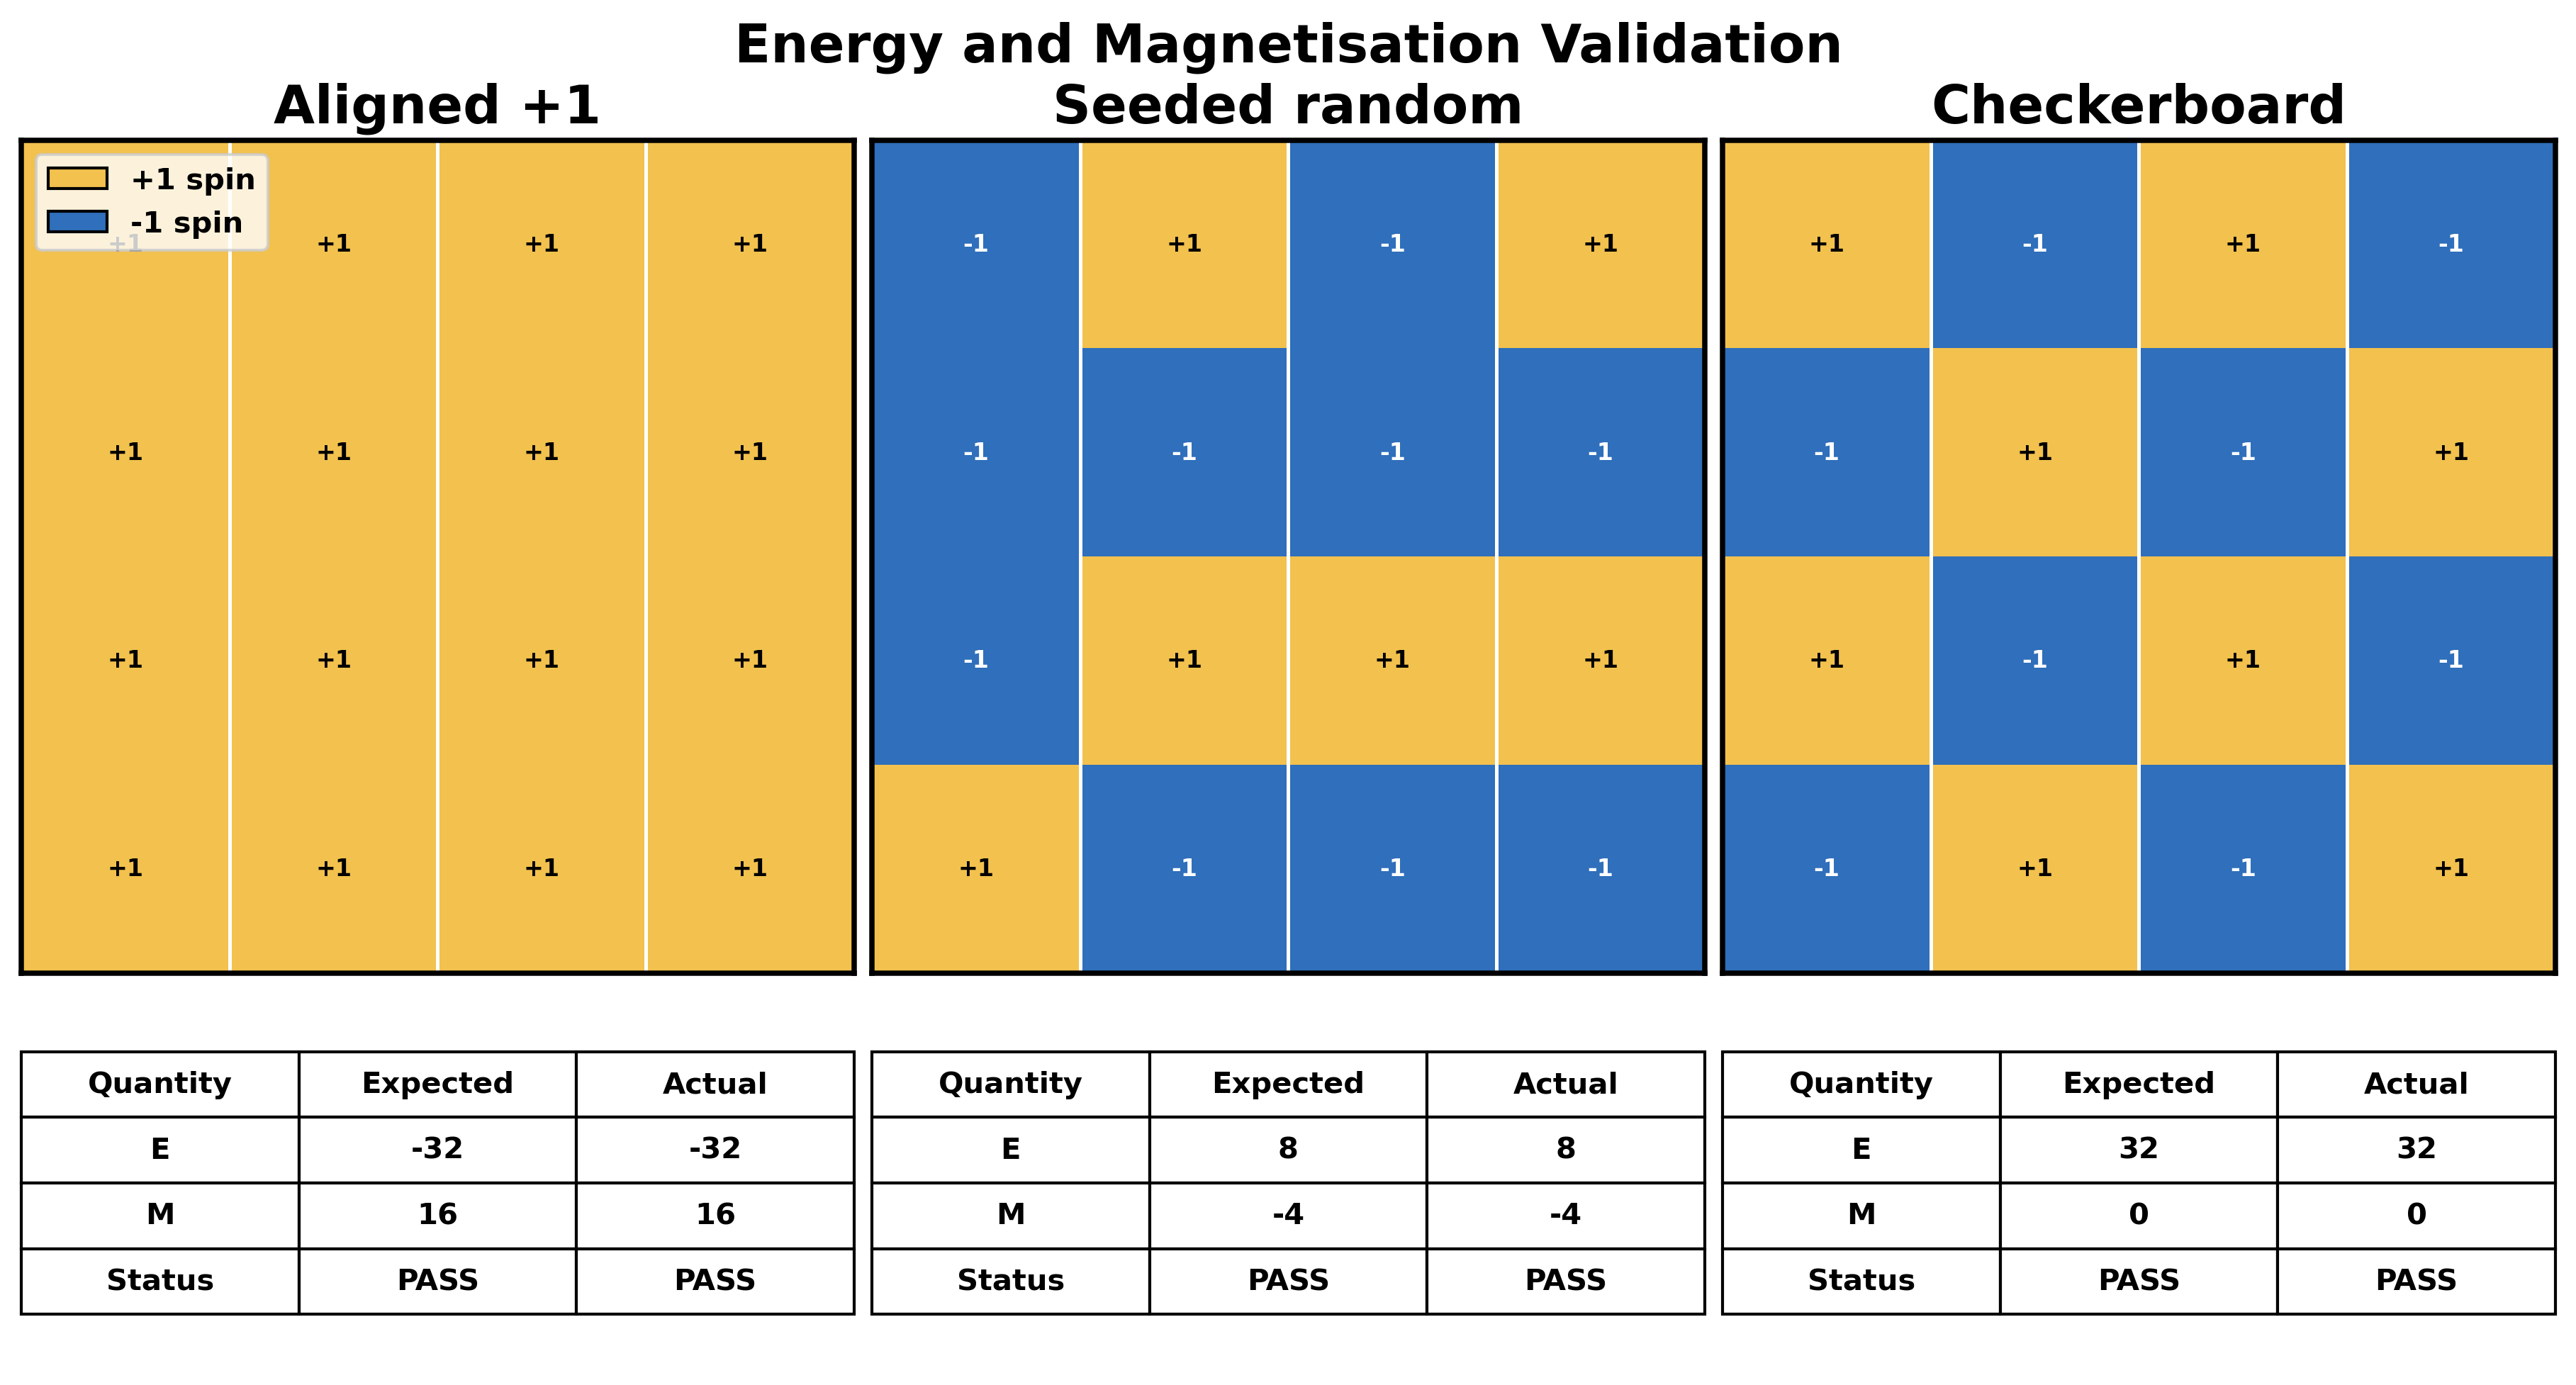
\includegraphics[width=0.82\textwidth]{figures/fig_section2_validation.png}
  \caption{Exact validation configurations confirm the periodic-boundary energy and magnetisation calculations. The aligned, seeded-random and checkerboard \(4 \times 4\) lattices test the ground-state limit, non-trivial wrapping and the antialigned bond limit.}
  \label{fig:si_validation}
\end{figure}

\clearpage
\begin{figure}[p]
  \centering
  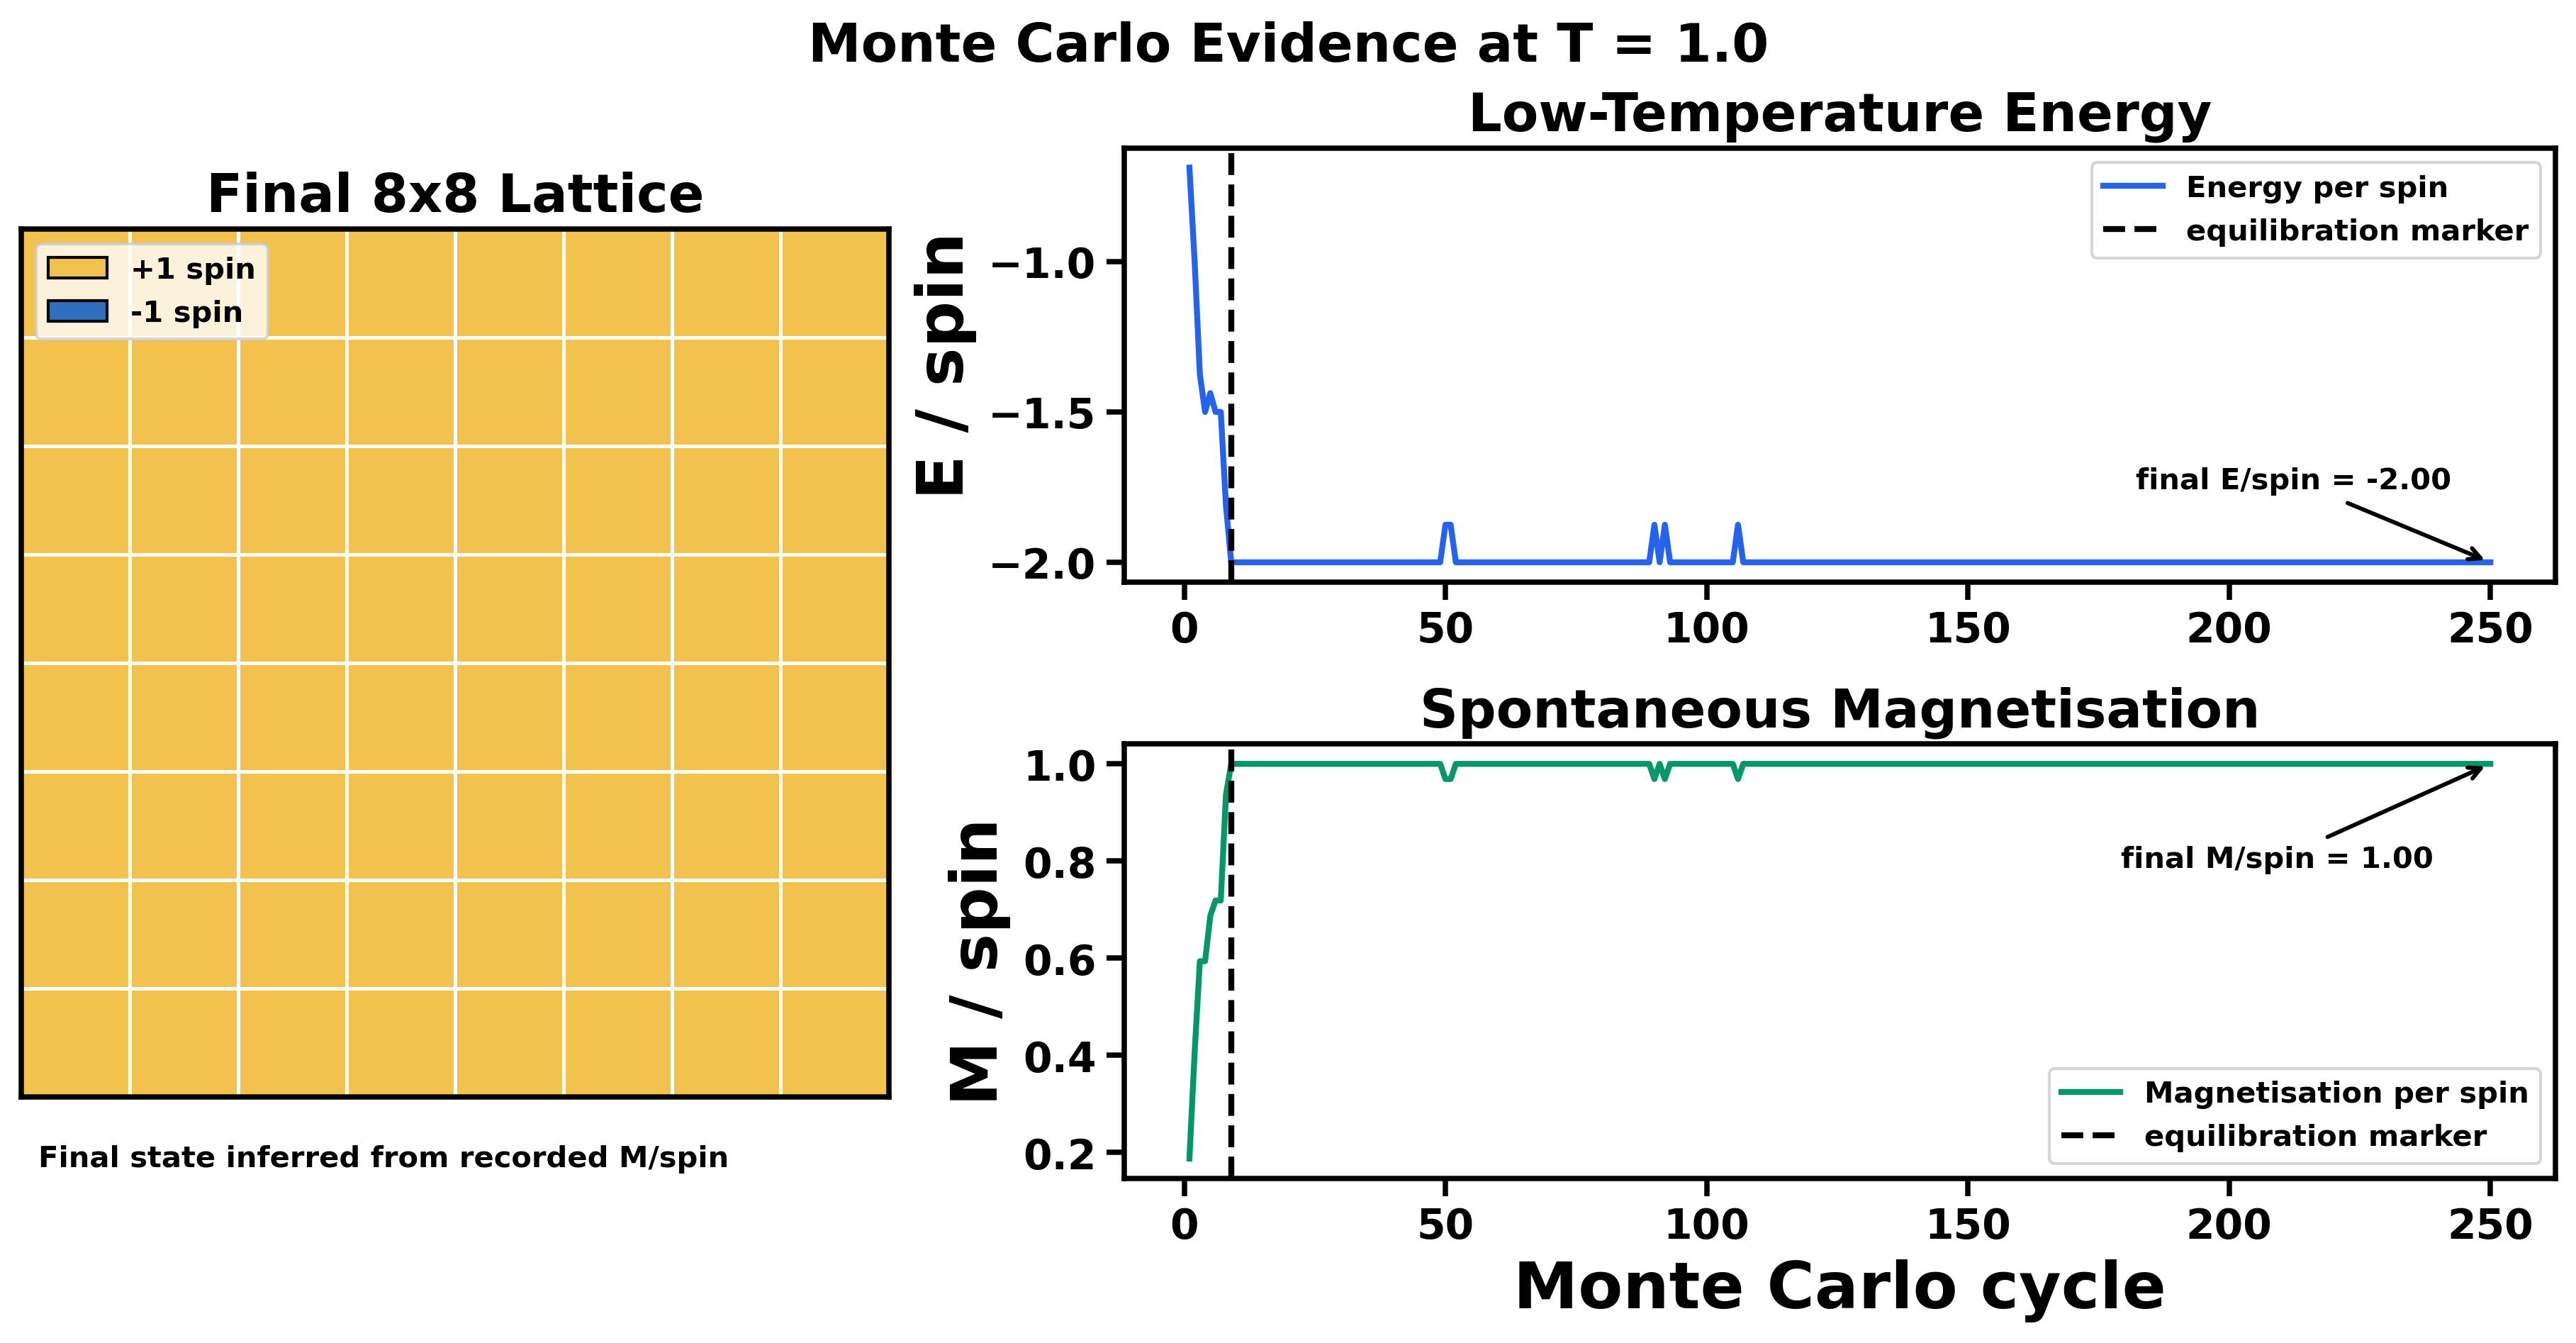
\includegraphics[width=0.86\textwidth]{figures/fig_section3_low_temperature.png}
  \caption{The \(8 \times 8\) lattice reaches the fully ordered state at \(T=1.0\). The trajectory provides a low-temperature ordering check, not a guarantee of rapid equilibration near \(T_C\).}
  \label{fig:si_lowtemp}
\end{figure}

\clearpage
\begin{figure}[p]
  \centering
  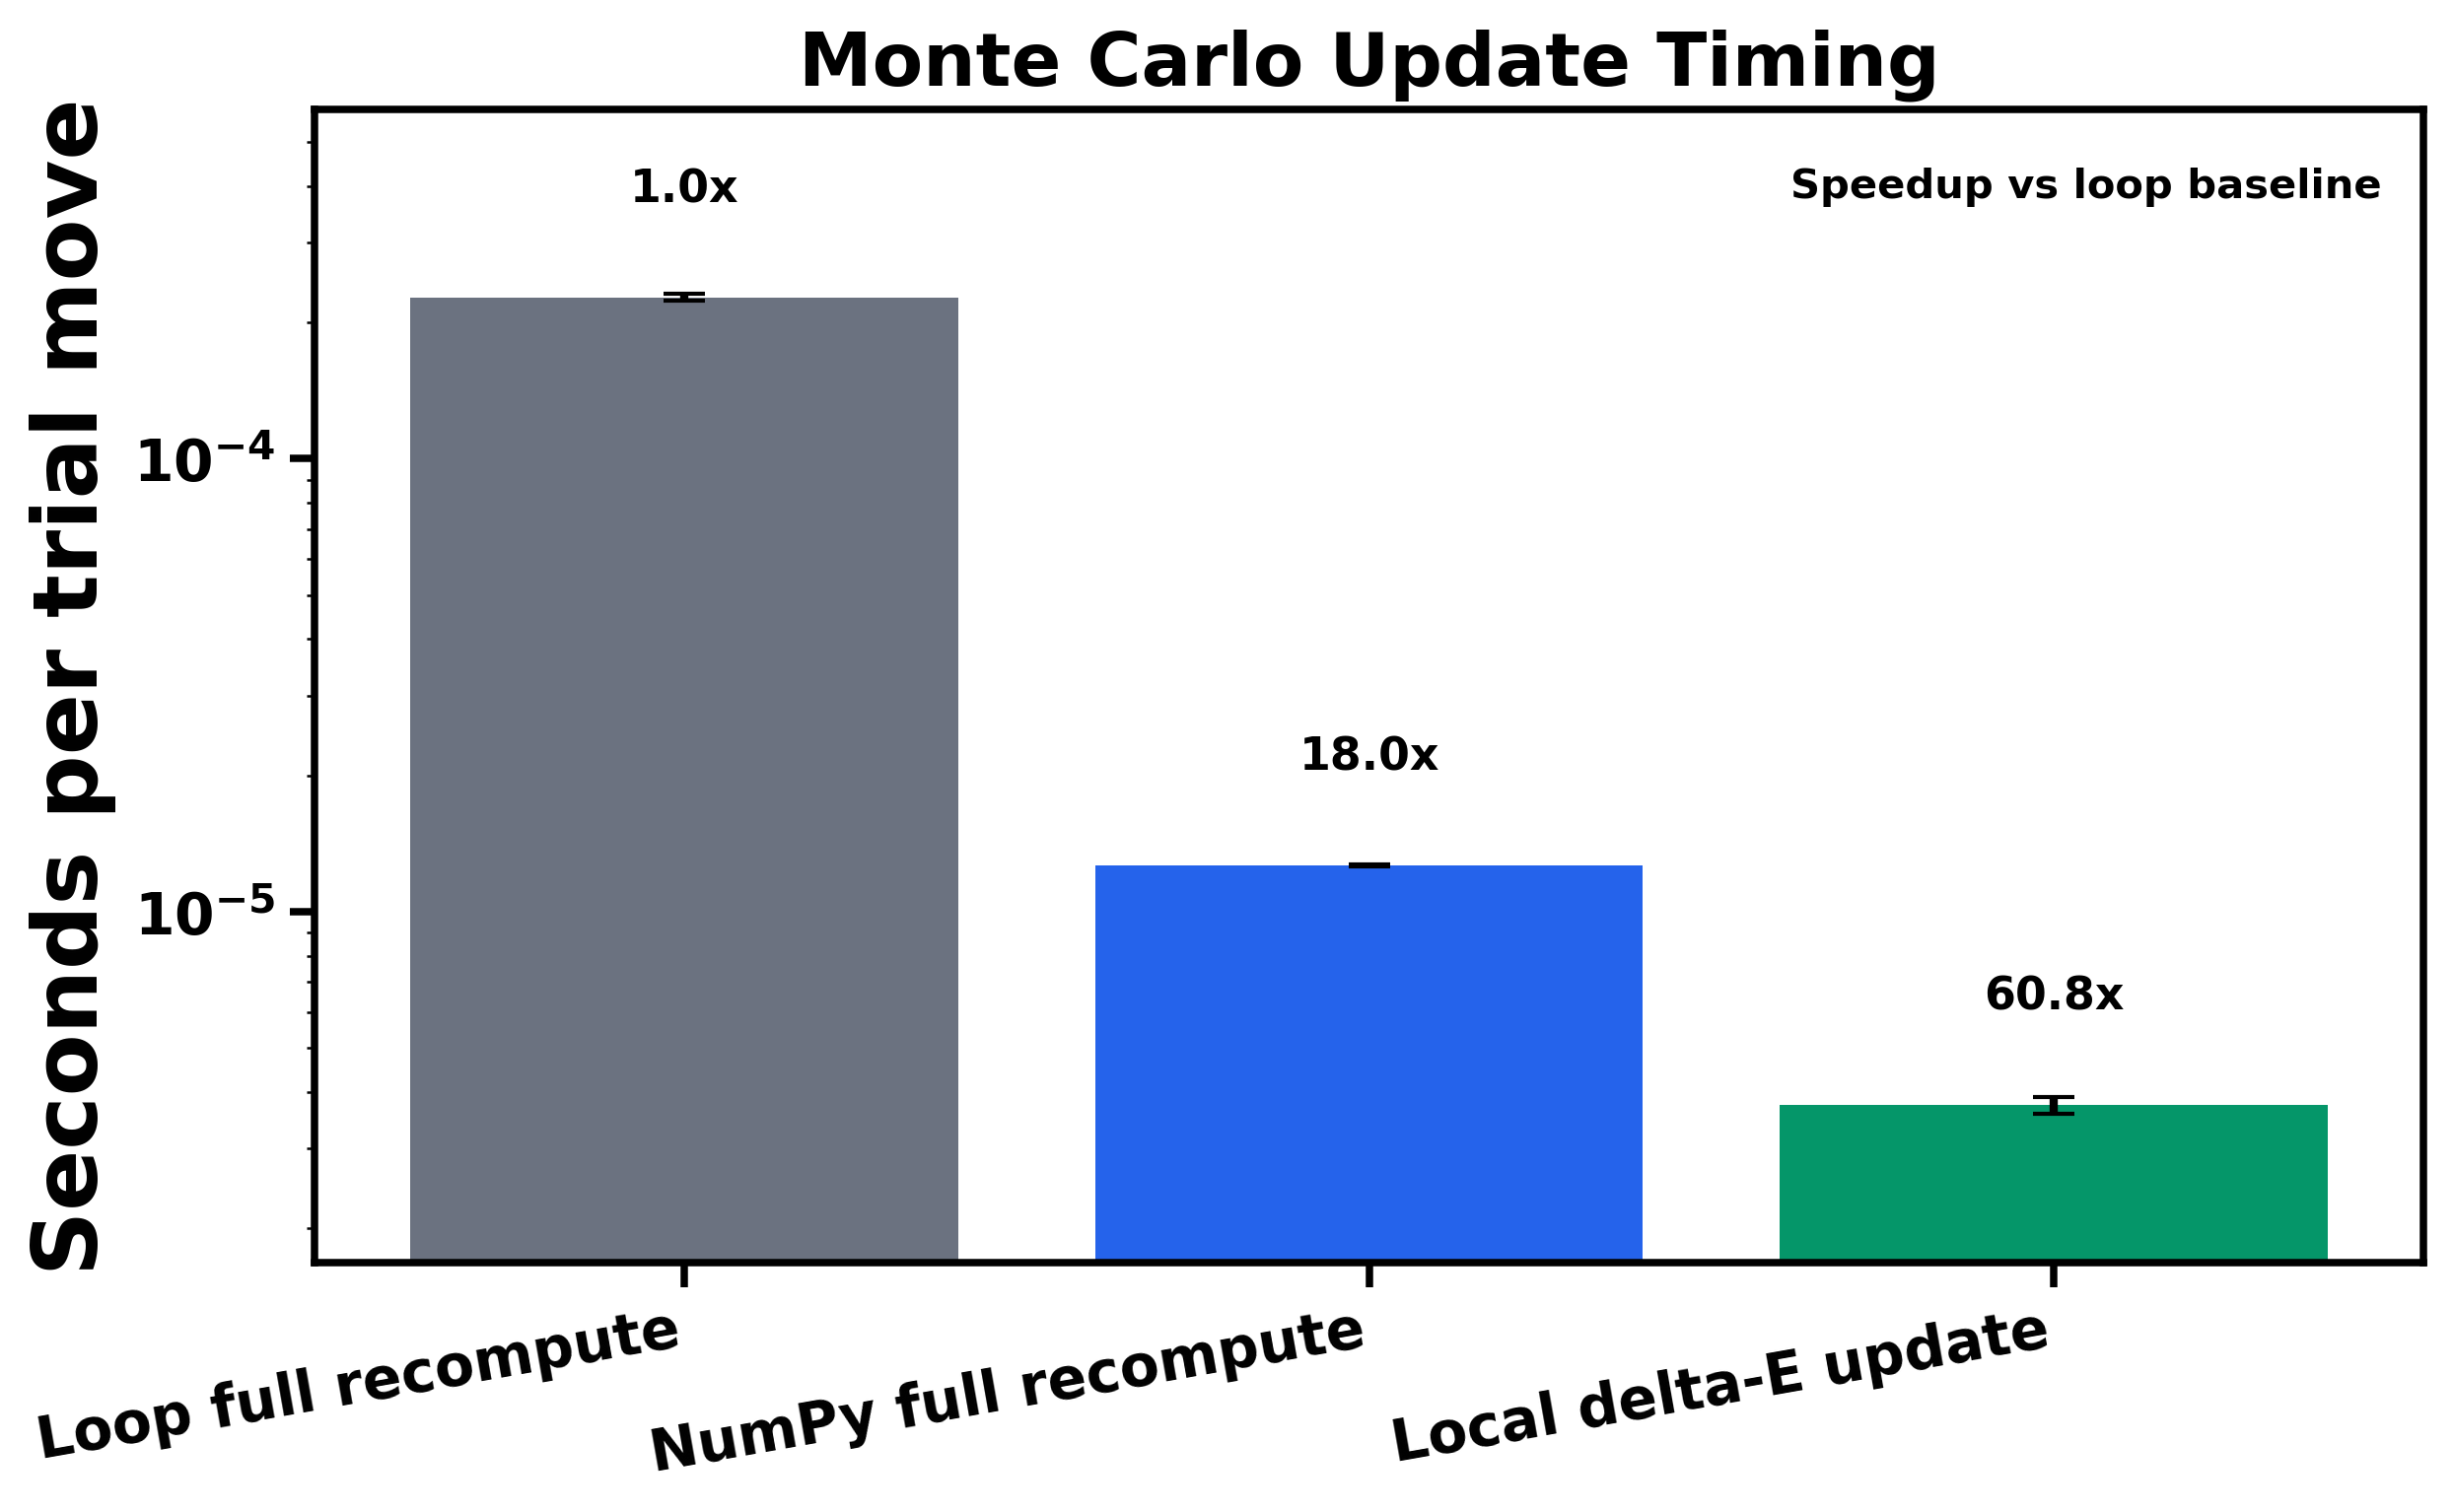
\includegraphics[width=0.68\textwidth]{figures/fig_section4_timing.png}
  \caption{The local \(\Delta E\) benchmark separates algorithmic improvement from NumPy vectorisation. Avoiding whole-lattice recomputation gives the largest speedup.}
  \label{fig:si_timing}
\end{figure}

\clearpage
\begin{figure}[p]
  \centering
  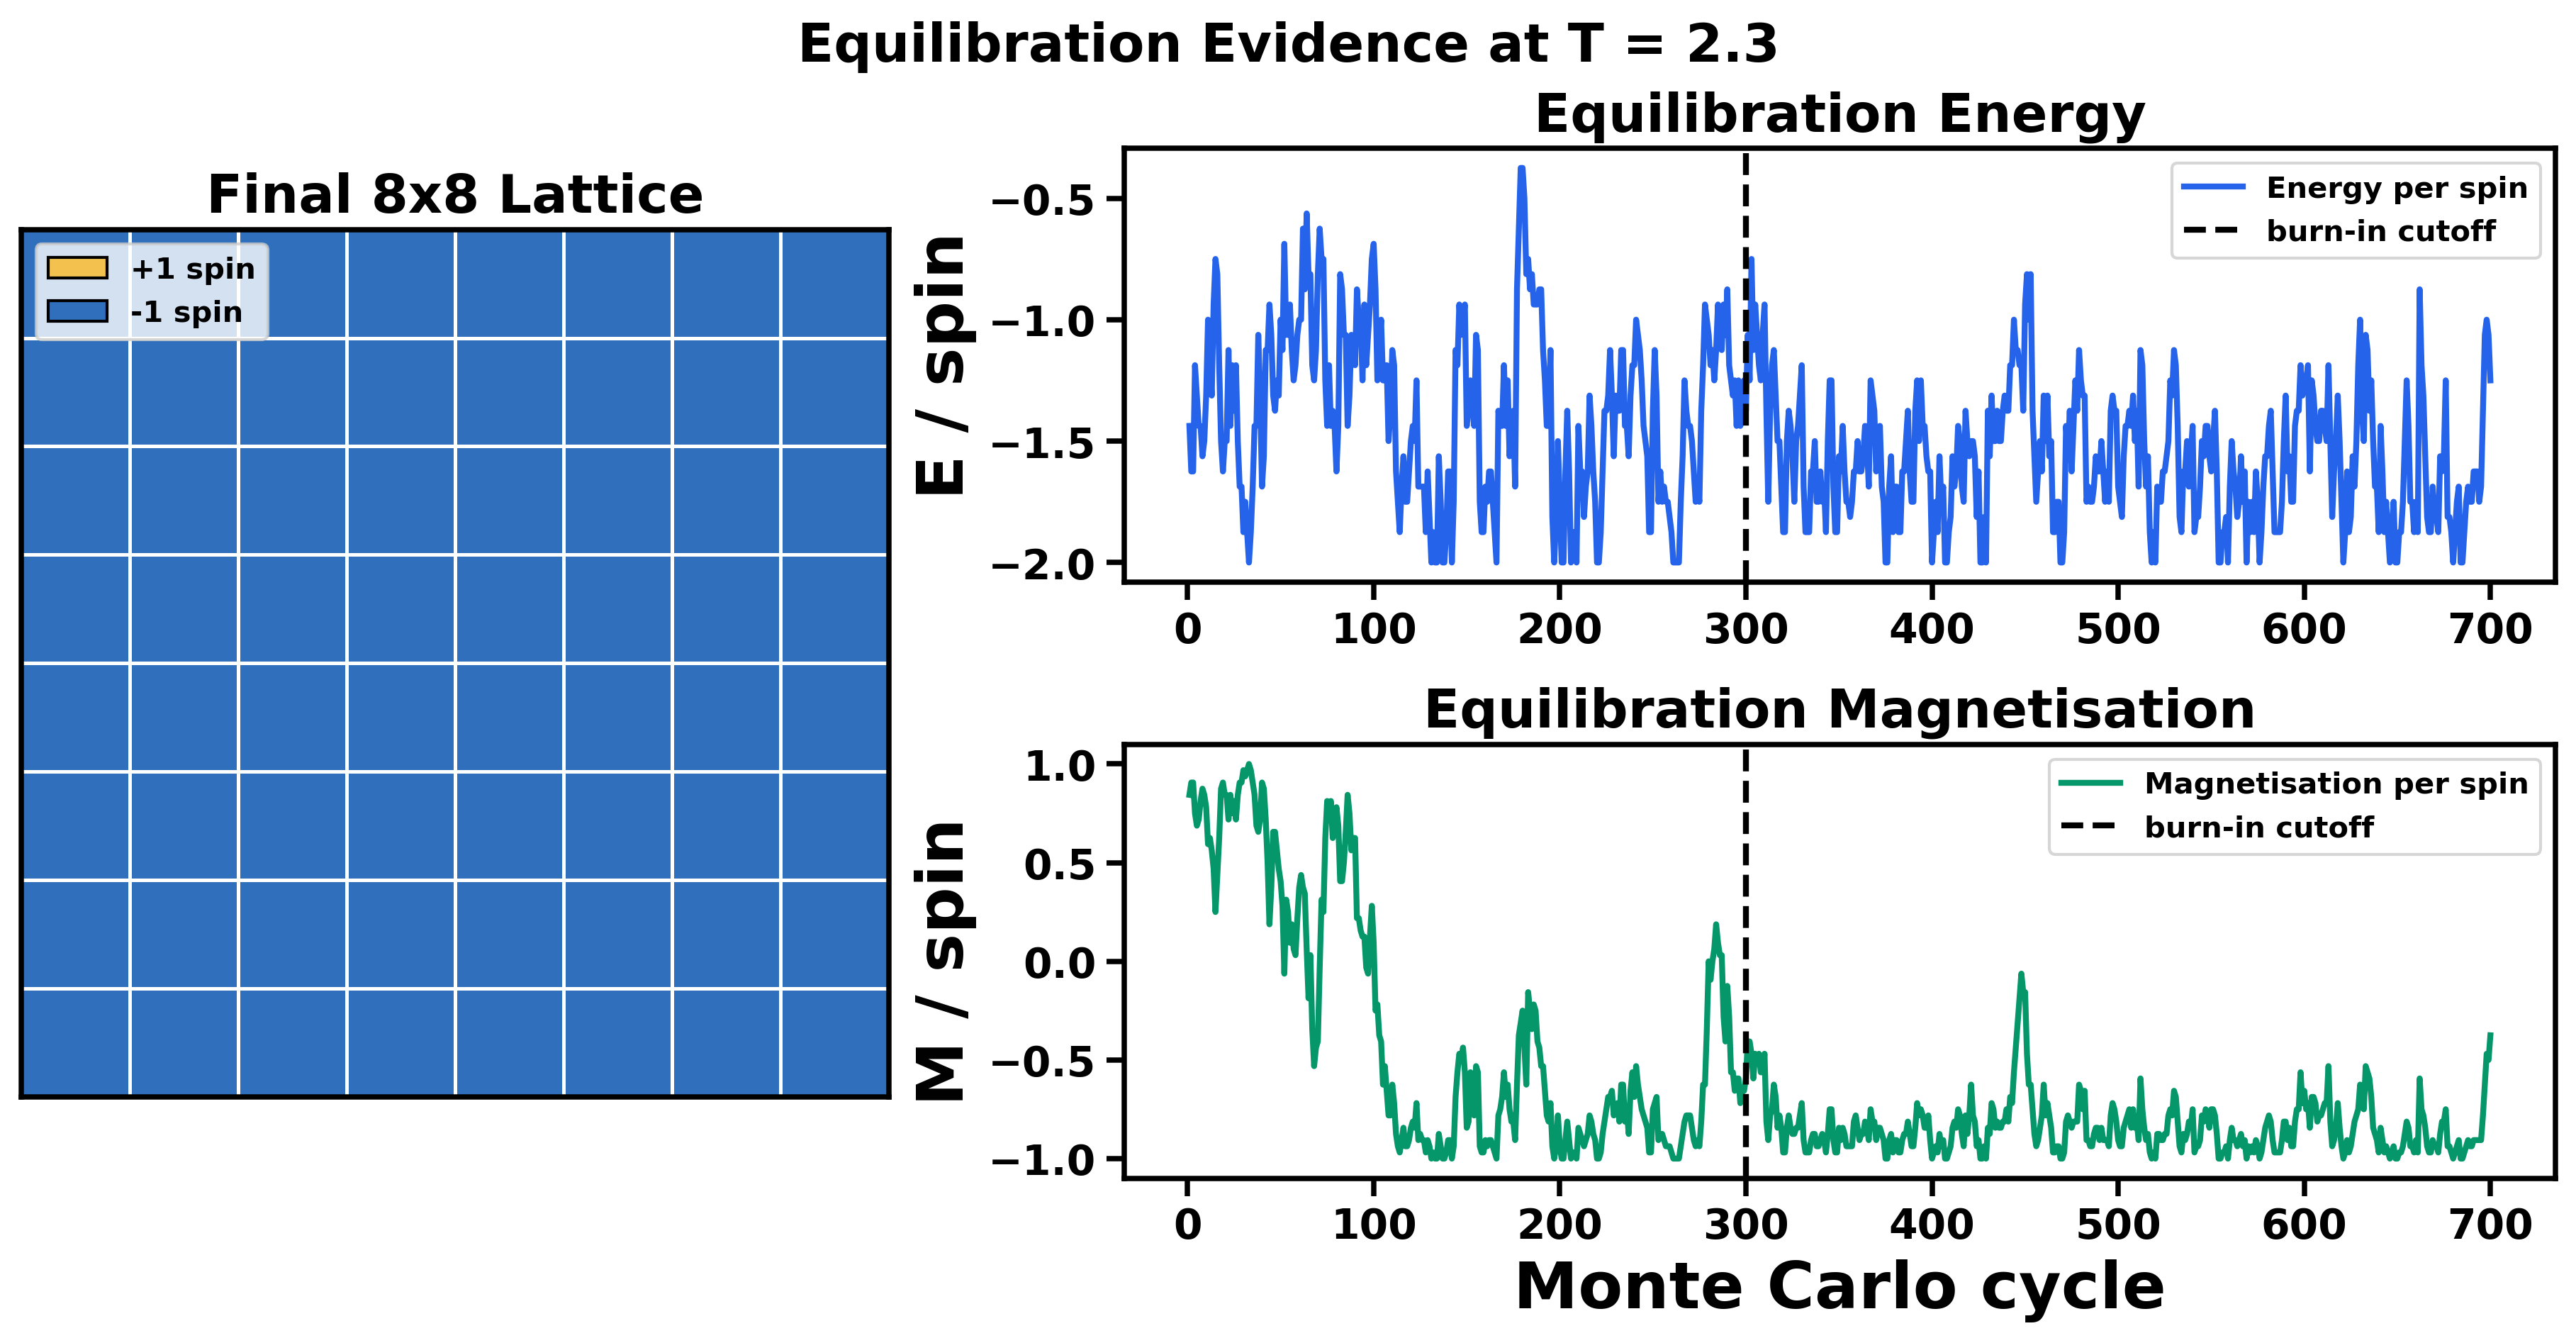
\includegraphics[width=0.86\textwidth]{figures/fig_section5_equilibration.png}
  \caption{The 300-cycle burn-in cut removes the main relaxation transient from the \(8 \times 8\) production statistics near \(T=2.3\).}
  \label{fig:si_equilibration}
\end{figure}

\clearpage
\begin{figure}[p]
  \centering
  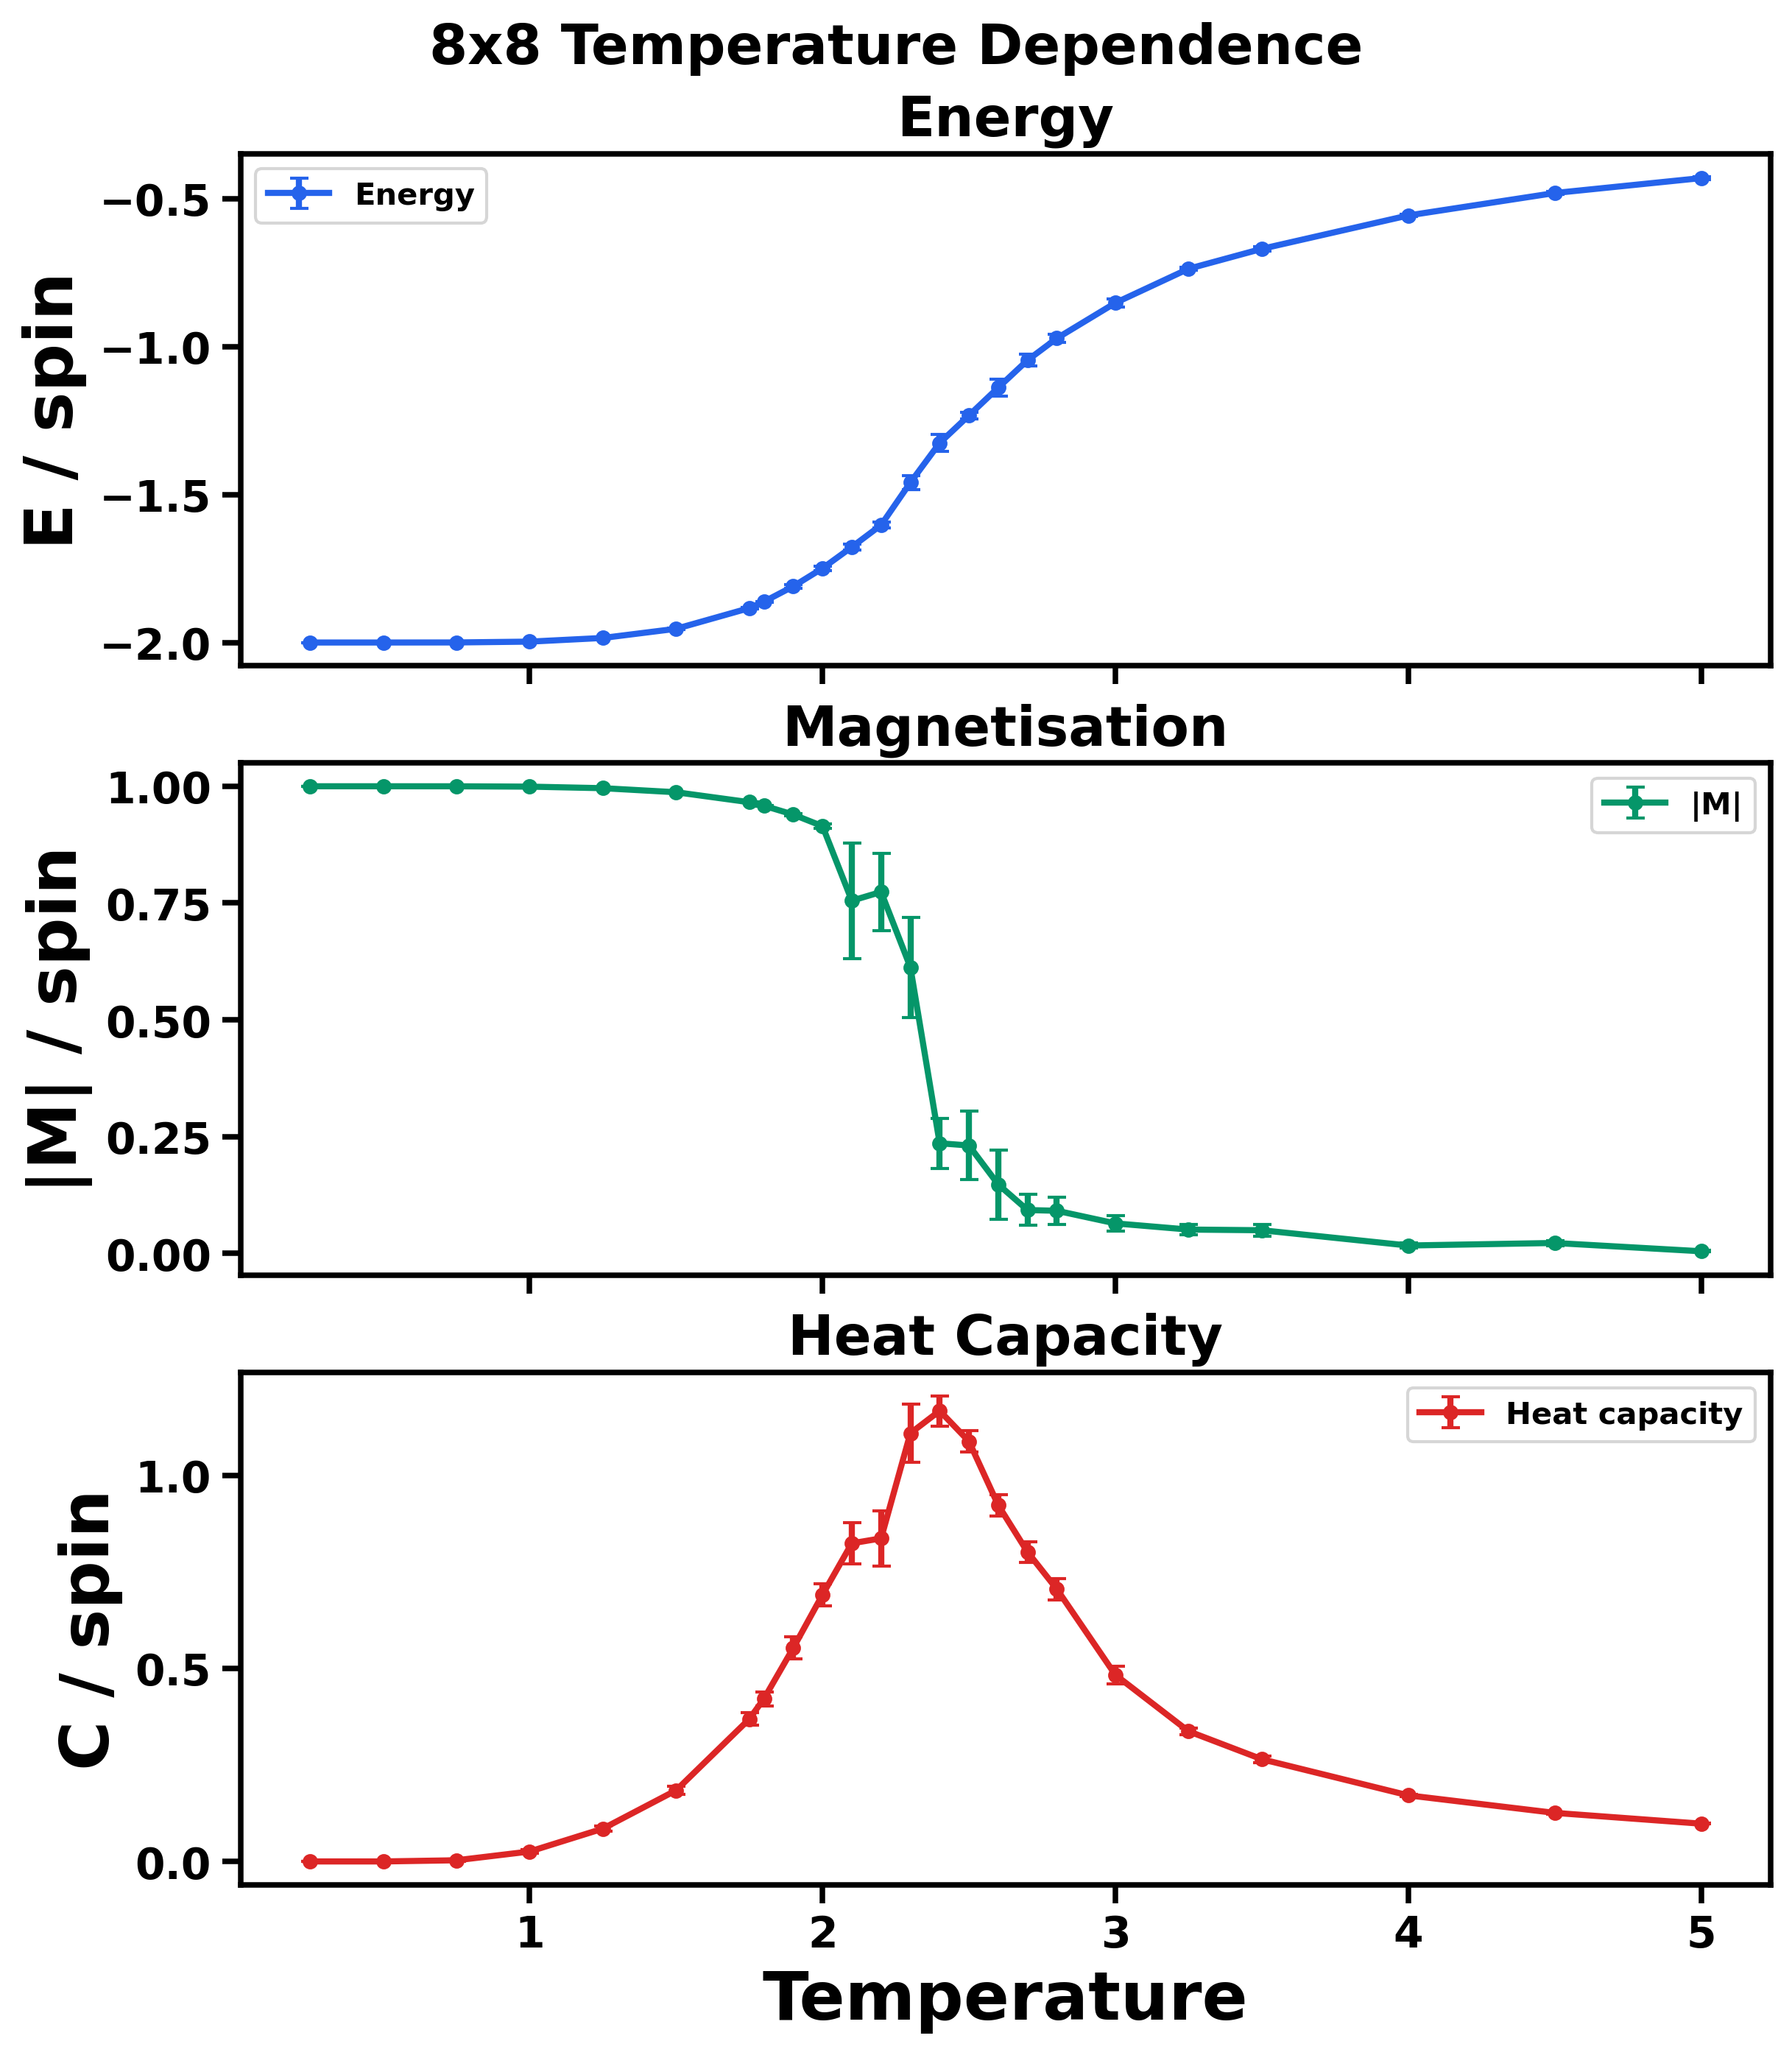
\includegraphics[width=0.82\textwidth]{figures/fig_section5_temperature_8x8.png}
  \caption{The \(8 \times 8\) scan shows a finite-size disordering crossover. Energy rises, \(\langle |M|\rangle/N\) falls, and heat capacity peaks near the critical region.}
  \label{fig:si_temperature8}
\end{figure}

\clearpage
\begin{figure}[p]
  \centering
  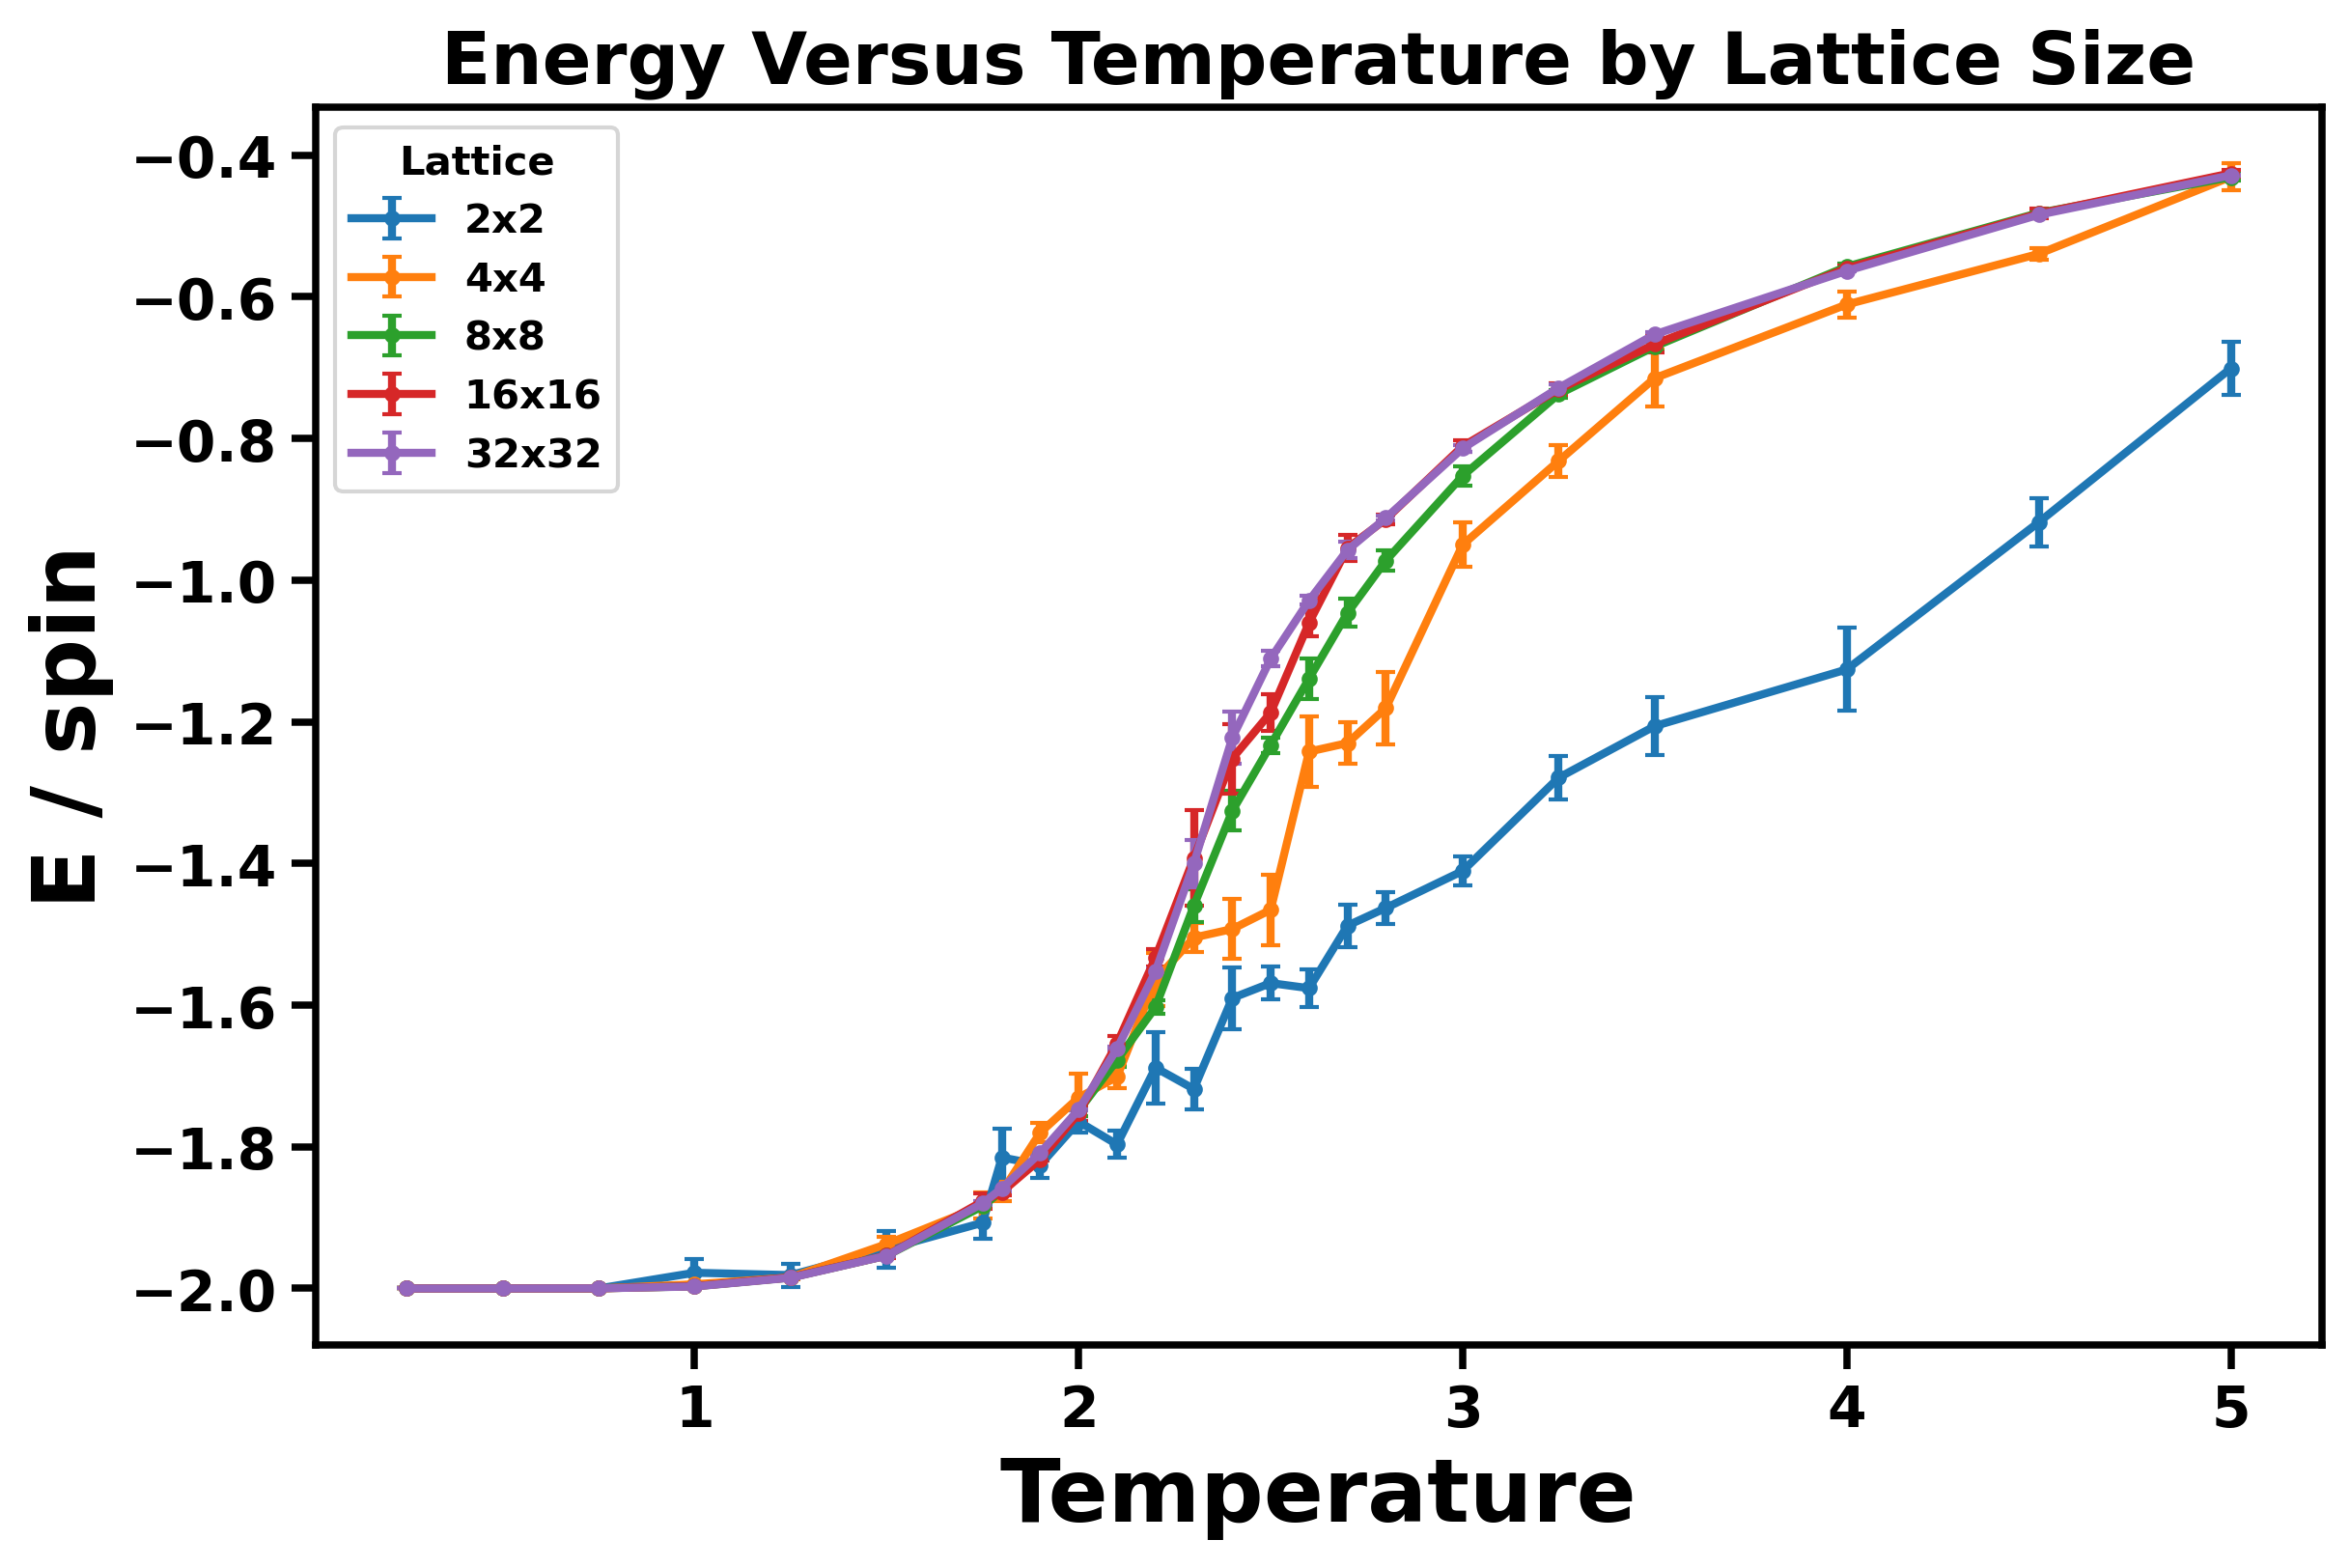
\includegraphics[width=0.86\textwidth]{figures/fig_section6_energy_size.png}
  \caption{Energy curves become most size-dependent in the critical region. Energy per spin is plotted for \(L=2,4,8,16,32\).}
  \label{fig:si_energy_size}
\end{figure}

\clearpage
\begin{figure}[p]
  \centering
  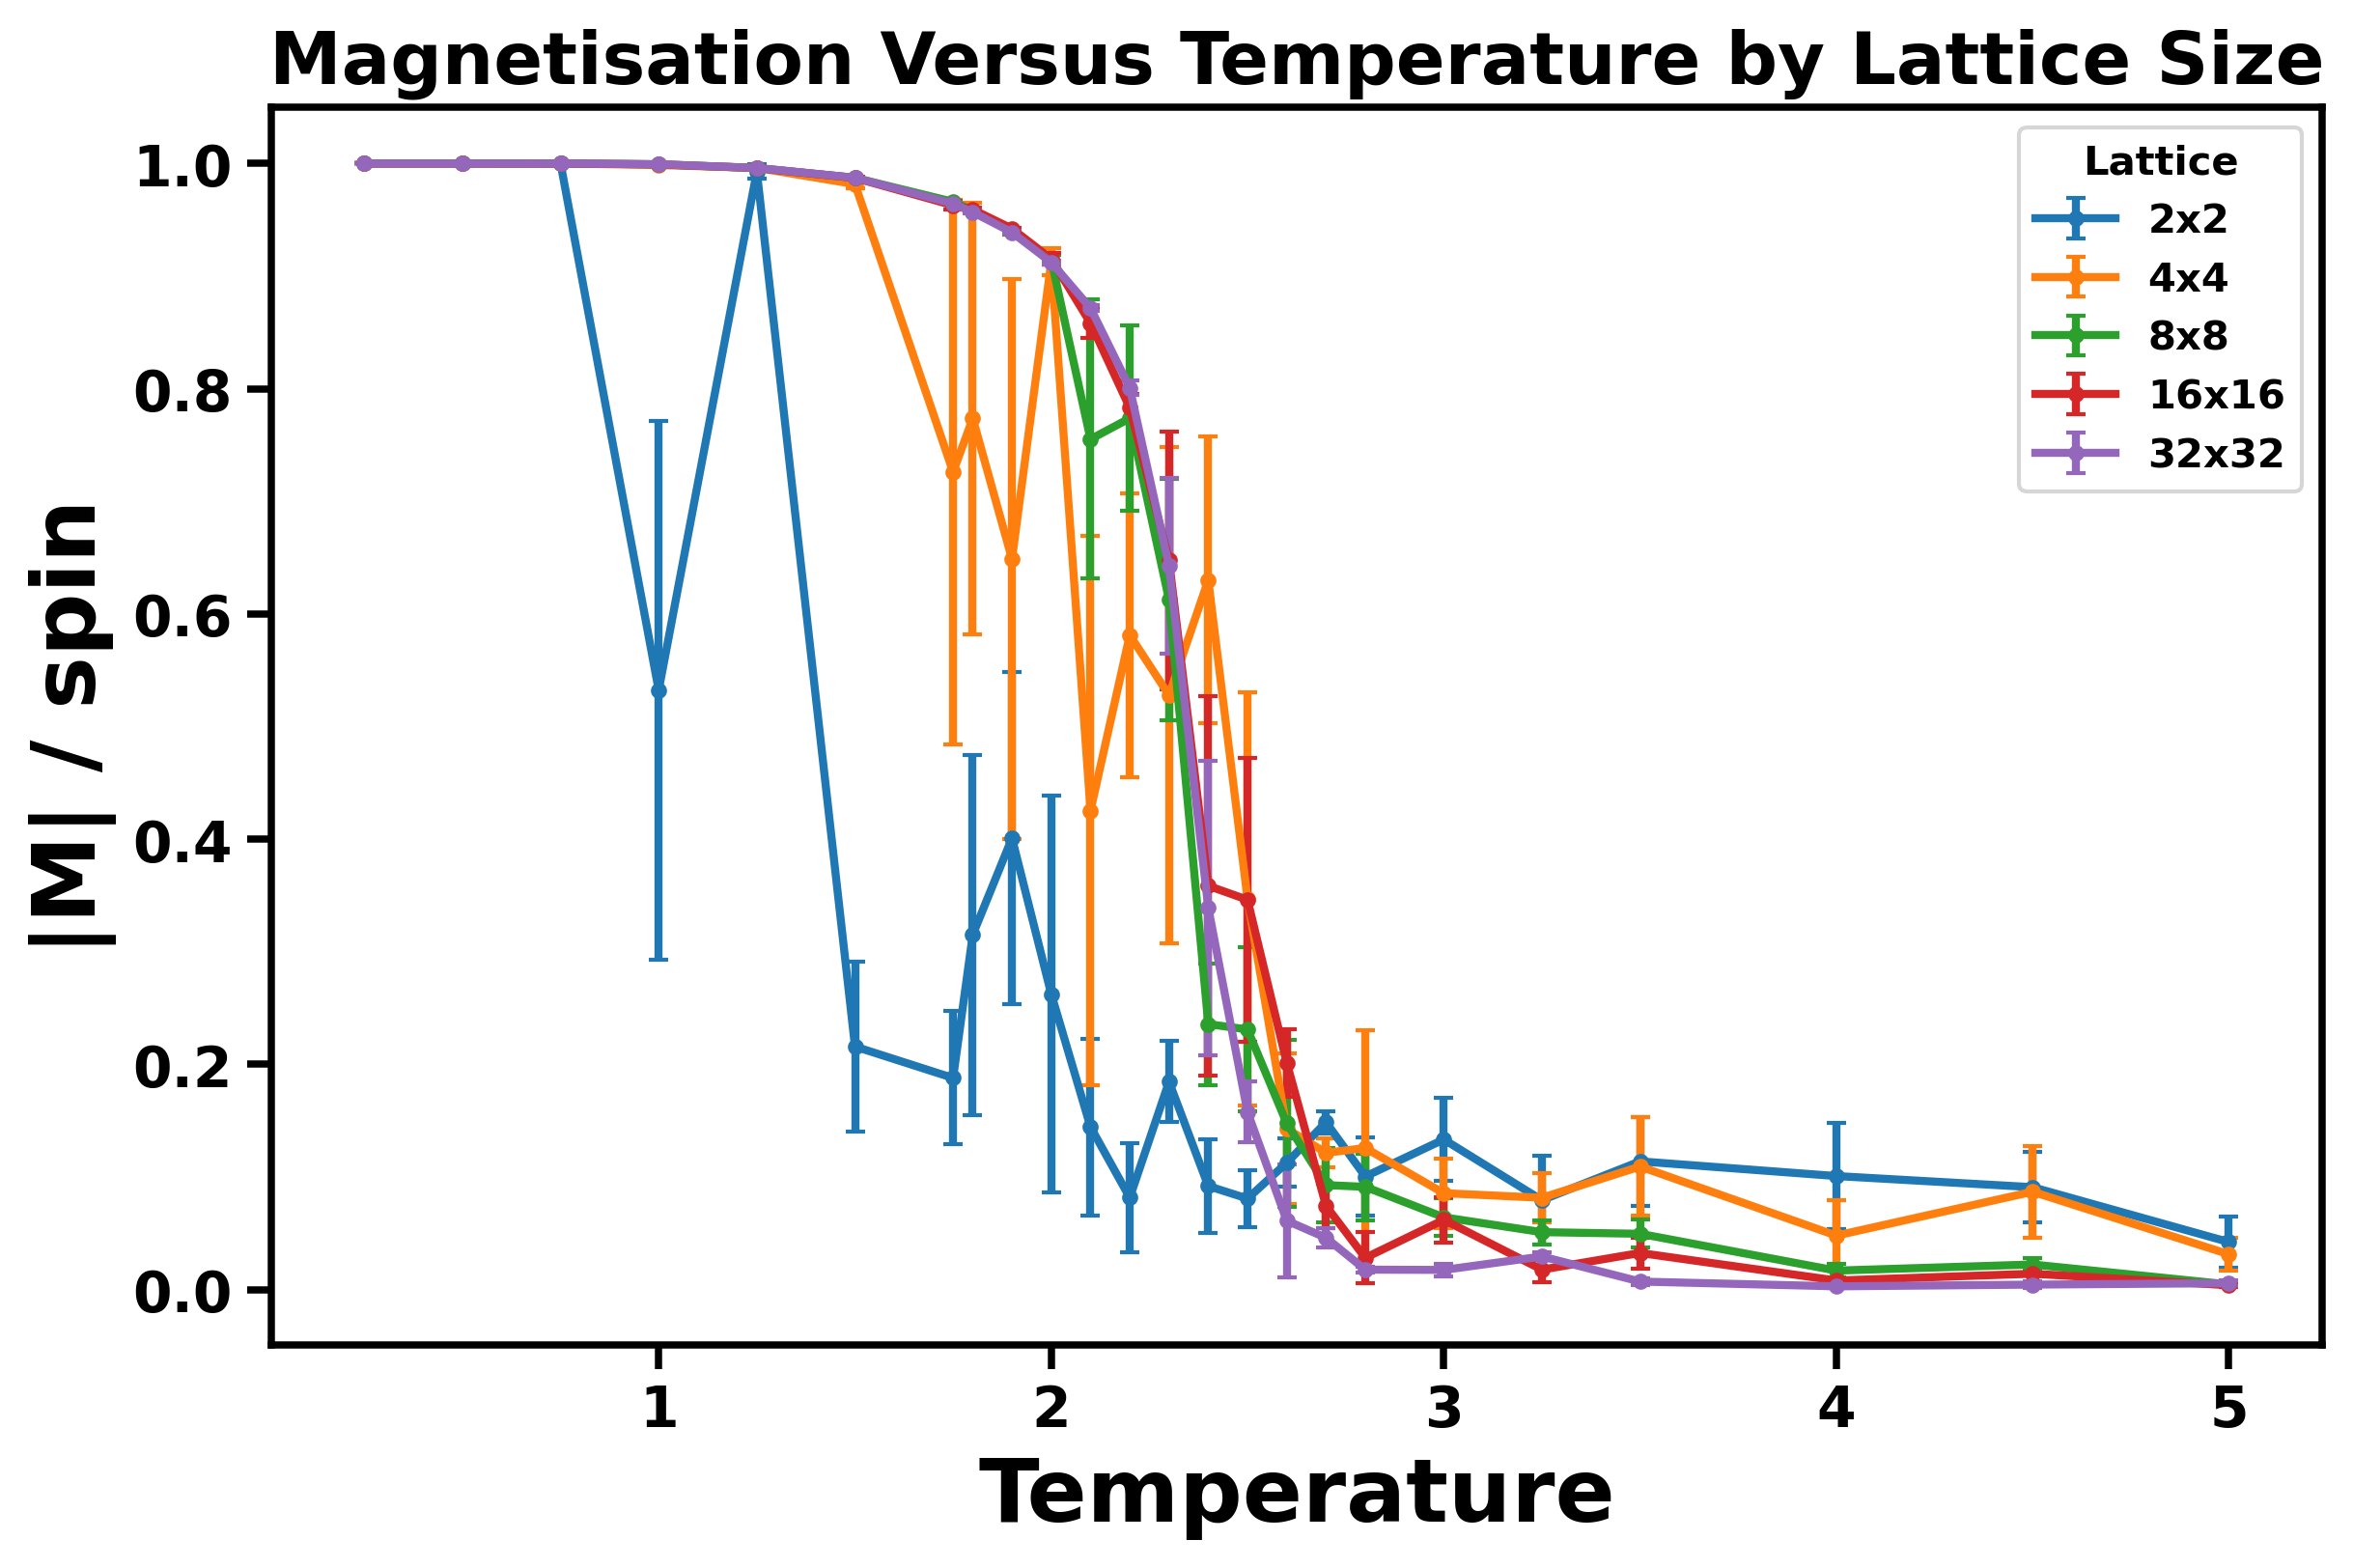
\includegraphics[width=0.86\textwidth]{figures/fig_section6_magnetisation_size.png}
  \caption{Larger lattices show a sharper loss of magnetisation near the transition. Absolute magnetisation per spin is plotted for \(L=2,4,8,16,32\).}
  \label{fig:si_mag_size}
\end{figure}

\clearpage
\begin{figure}[p]
  \centering
  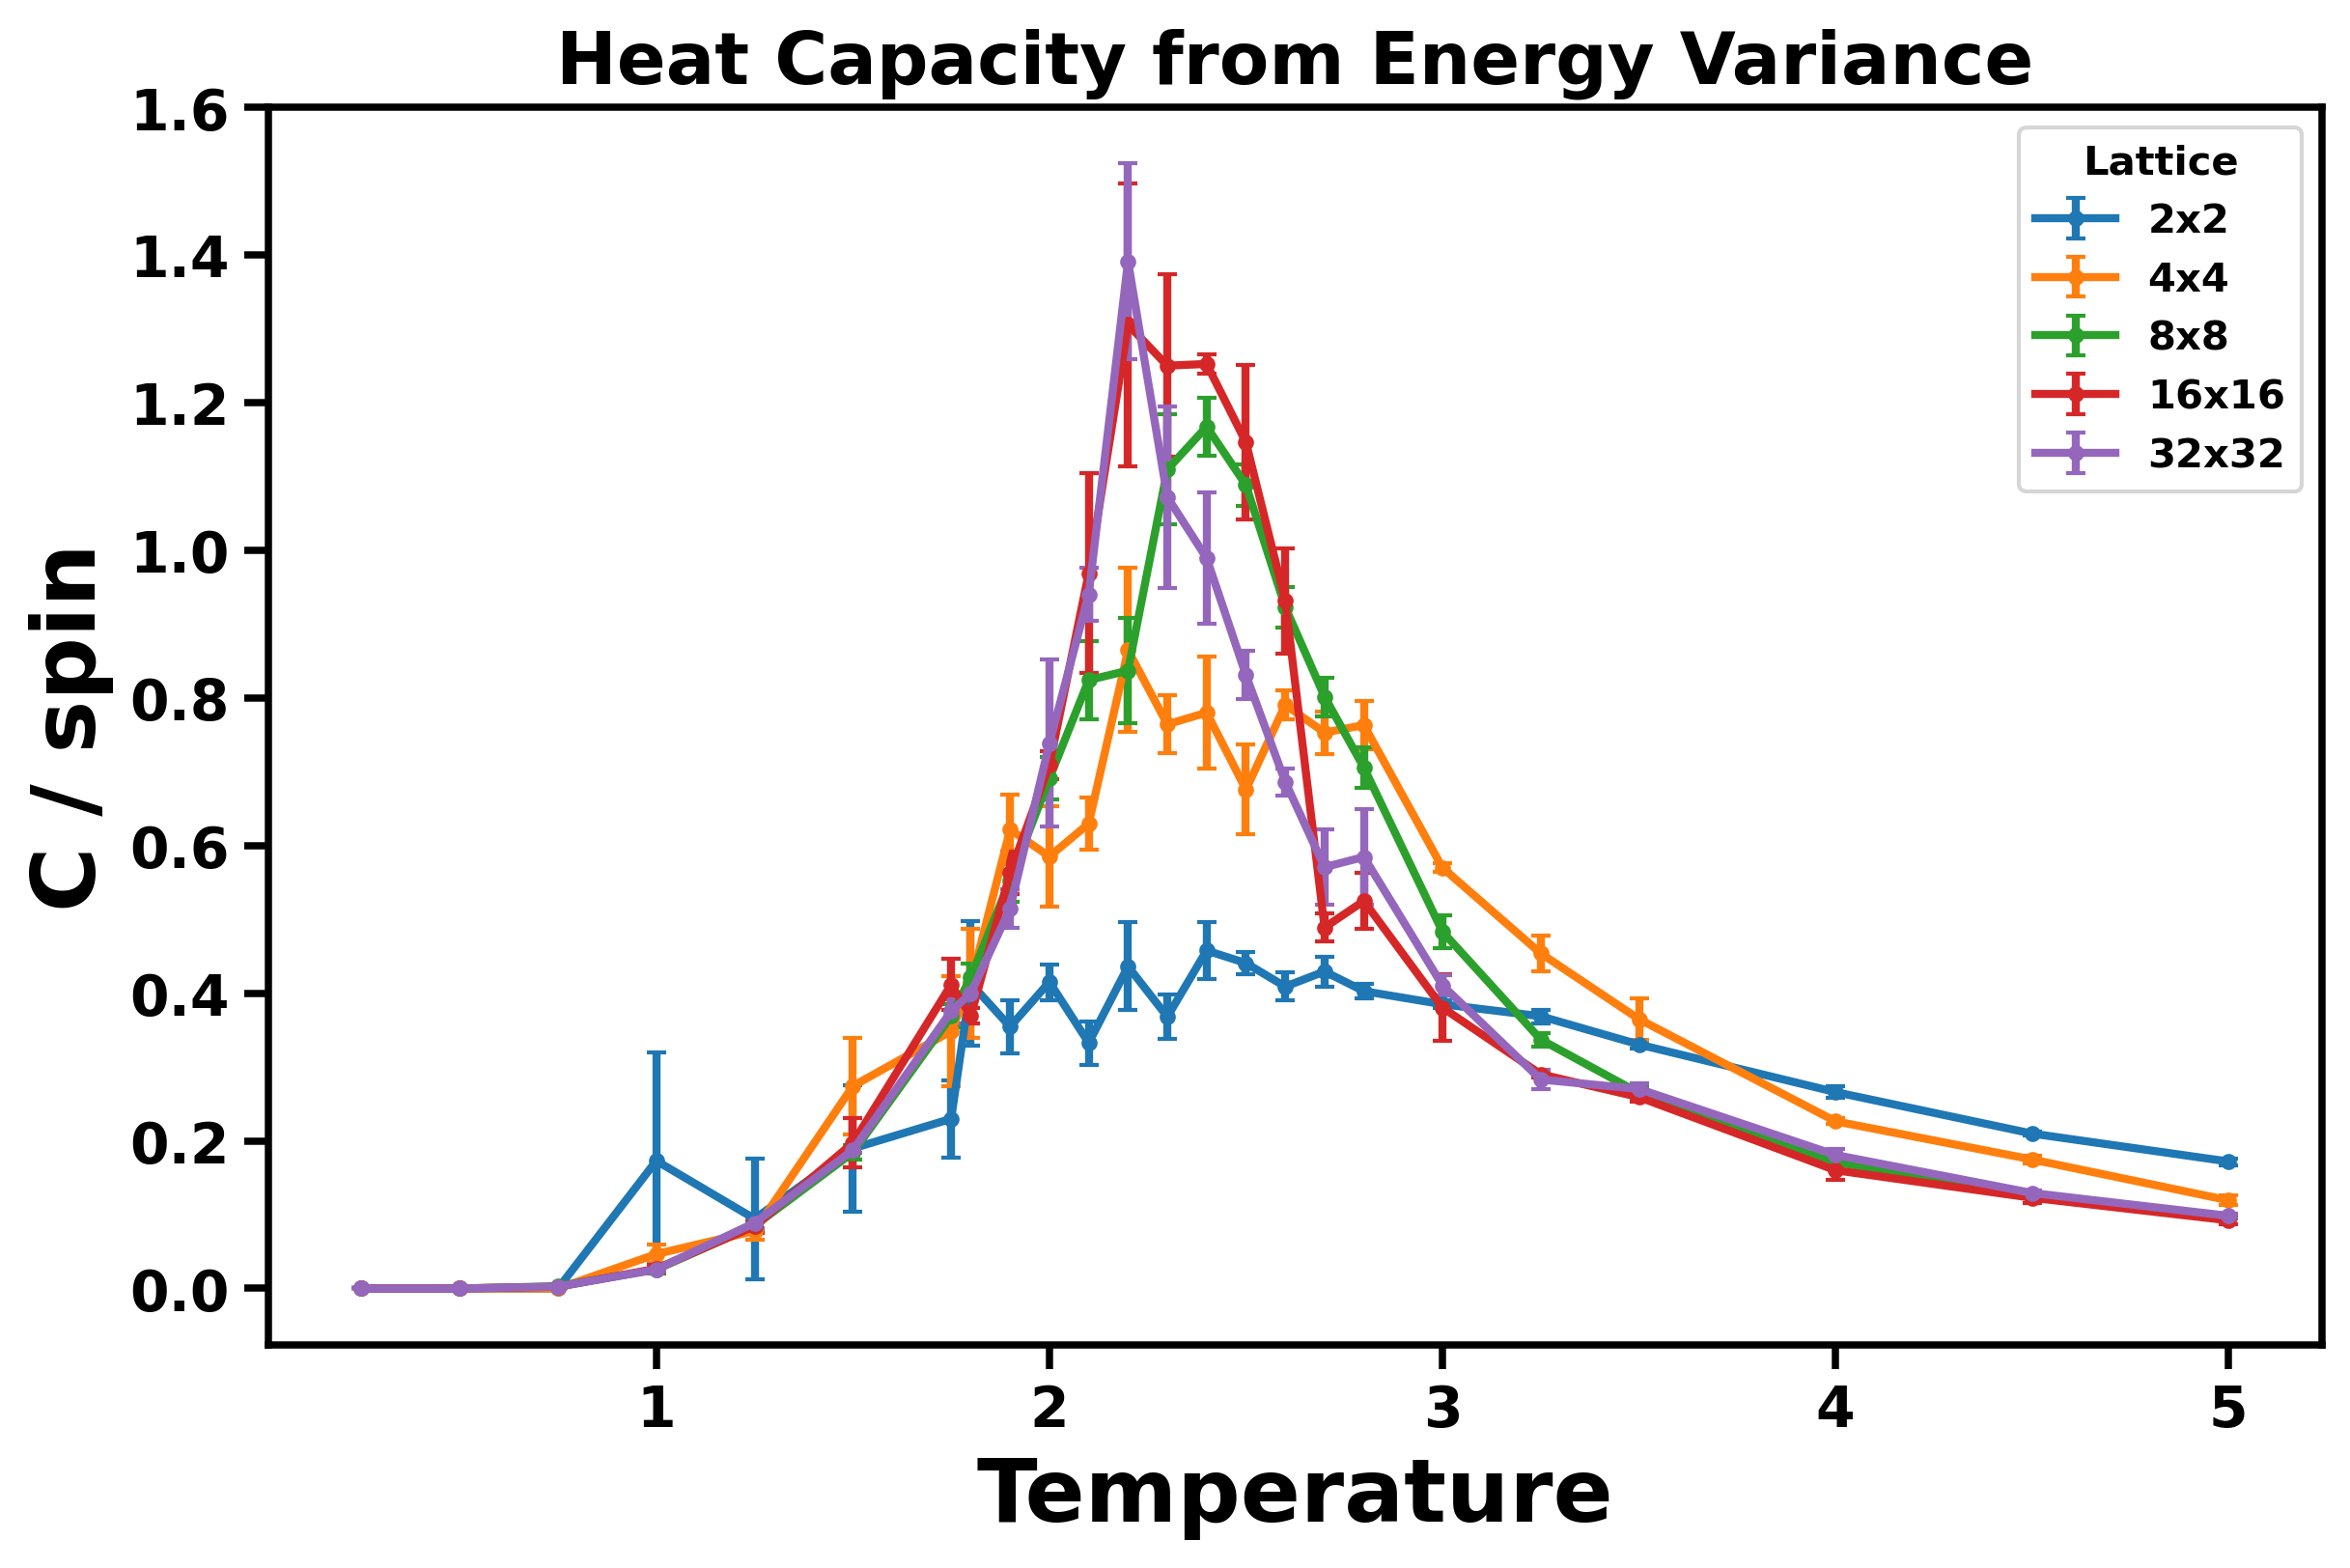
\includegraphics[width=0.84\textwidth]{figures/fig_section7_heat_capacity.png}
  \caption{Heat-capacity peaks grow and sharpen with lattice size. The increasing \(C/N\) peak height is consistent with stronger critical energy fluctuations as the simulated system approaches the thermodynamic limit.}
  \label{fig:si_heat_capacity}
\end{figure}

\clearpage
\begin{figure}[p]
  \centering
  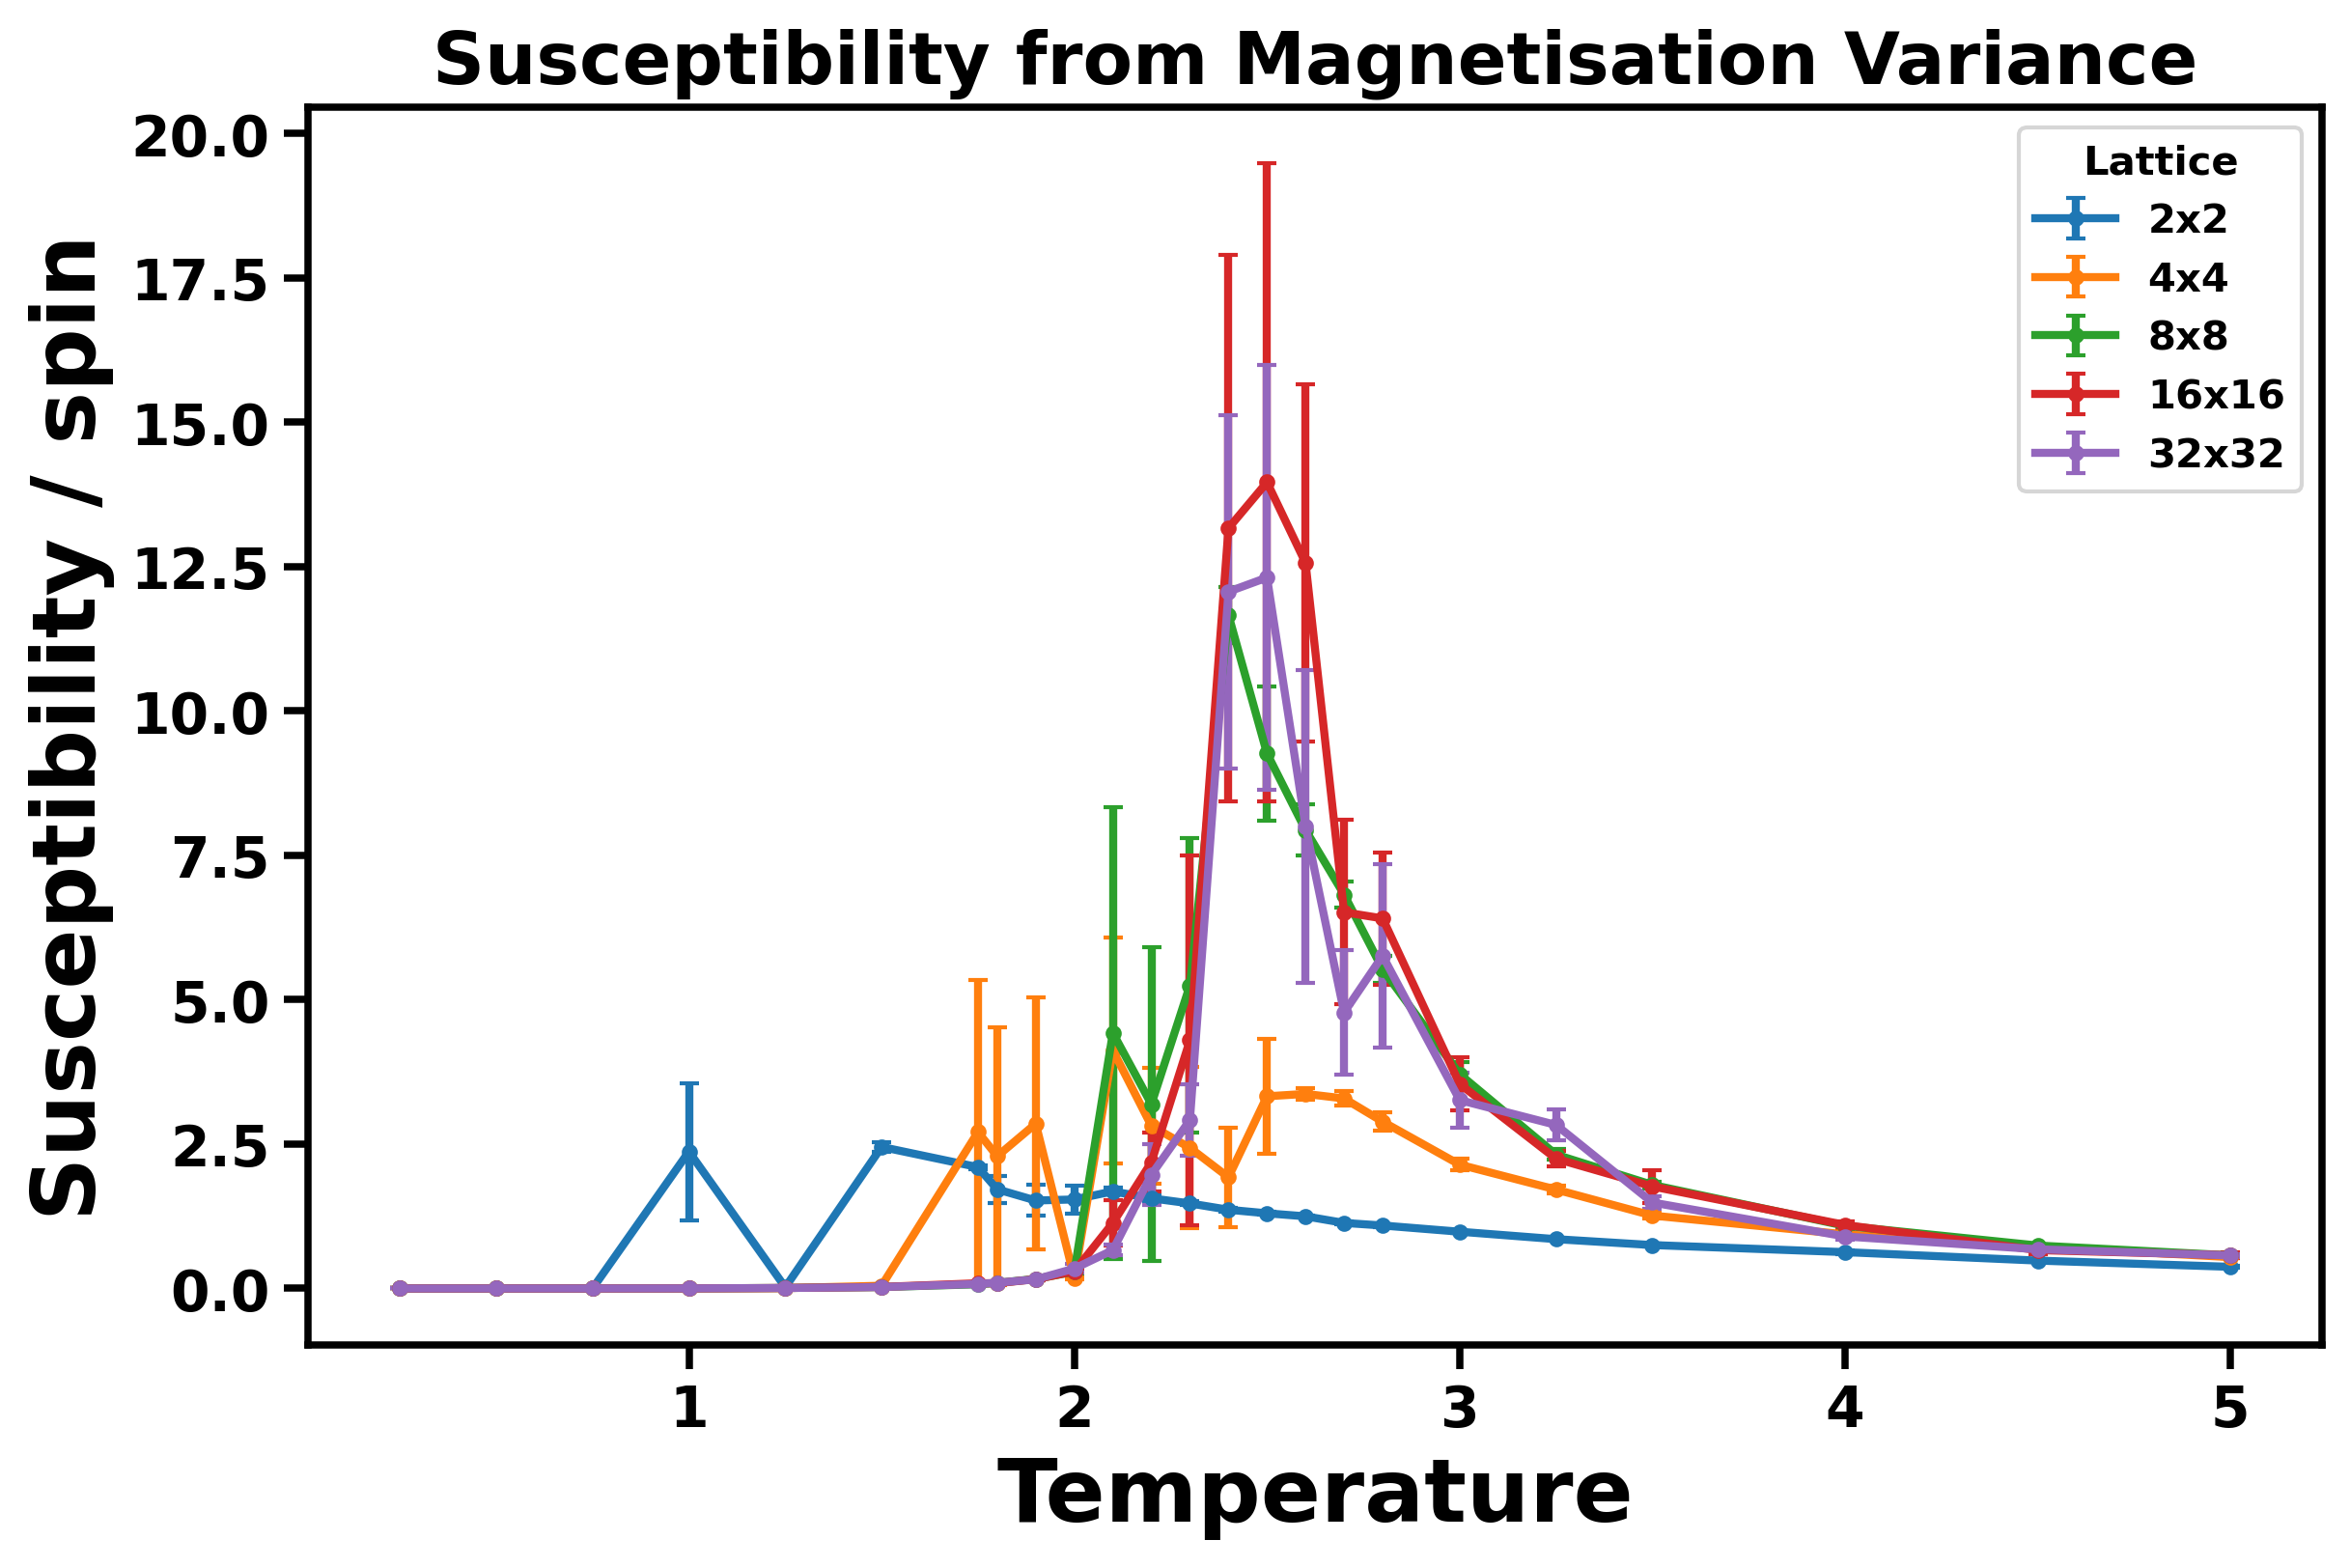
\includegraphics[width=0.84\textwidth]{figures/fig_section7_susceptibility.png}
  \caption{Susceptibility peaks in the critical region but is noisier than heat capacity. \(\chi/N\) is plotted for all simulated lattice sizes using signed-\(M\) variance.}
  \label{fig:si_susceptibility}
\end{figure}

\clearpage
\begin{table}[H]
  \centering
  \begin{minipage}{0.58\textwidth}
    \captionsetup{justification=centering,singlelinecheck=true,width=\linewidth}
    \caption{Short-run response-function peak locations are grid-limited and non-monotonic.}
    \label{tab:si_shortpeaks}
    \centering
    \begin{tabular}{cccc}
      \toprule
      \(L\) & \(T_{\max}(C)\) & \(C_{\max}/N\) & \(T_{\max}(\chi)\) \\
      \midrule
      2  & 2.4 & 0.458 & 1.5 \\
      4  & 2.2 & 0.865 & 2.1 \\
      8  & 2.4 & 1.167 & 2.4 \\
      16 & 2.2 & 1.305 & 2.5 \\
      32 & 2.2 & 1.391 & 2.5 \\
      \bottomrule
    \end{tabular}
  \end{minipage}
\end{table}

\begin{table}[H]
  \centering
  \begin{minipage}{0.74\textwidth}
    \captionsetup{justification=centering,singlelinecheck=true,width=\linewidth}
    \caption{Curie-temperature estimates from finite-size peak scaling. Polynomial peak fits used \(L=4,8,16,32\).}
    \label{tab:si_scaling}
    \centering
    \begin{tabular}{llccc}
      \toprule
      Data source & Observable & \(T_{C,\infty}\) & Exact \(T_C\) & Difference \\
      \midrule
      Short-run & Heat capacity & 2.07925 & 2.26919 & -0.18994 \\
      Short-run & Susceptibility & 2.46224 & 2.26919 & +0.19305 \\
      Reference & Heat capacity & 2.27592 & 2.26919 & +0.00673 \\
      Reference & Susceptibility & 2.44543 & 2.26919 & +0.17624 \\
      \bottomrule
    \end{tabular}
  \end{minipage}
\end{table}

\clearpage
\begin{figure}[p]
  \centering
  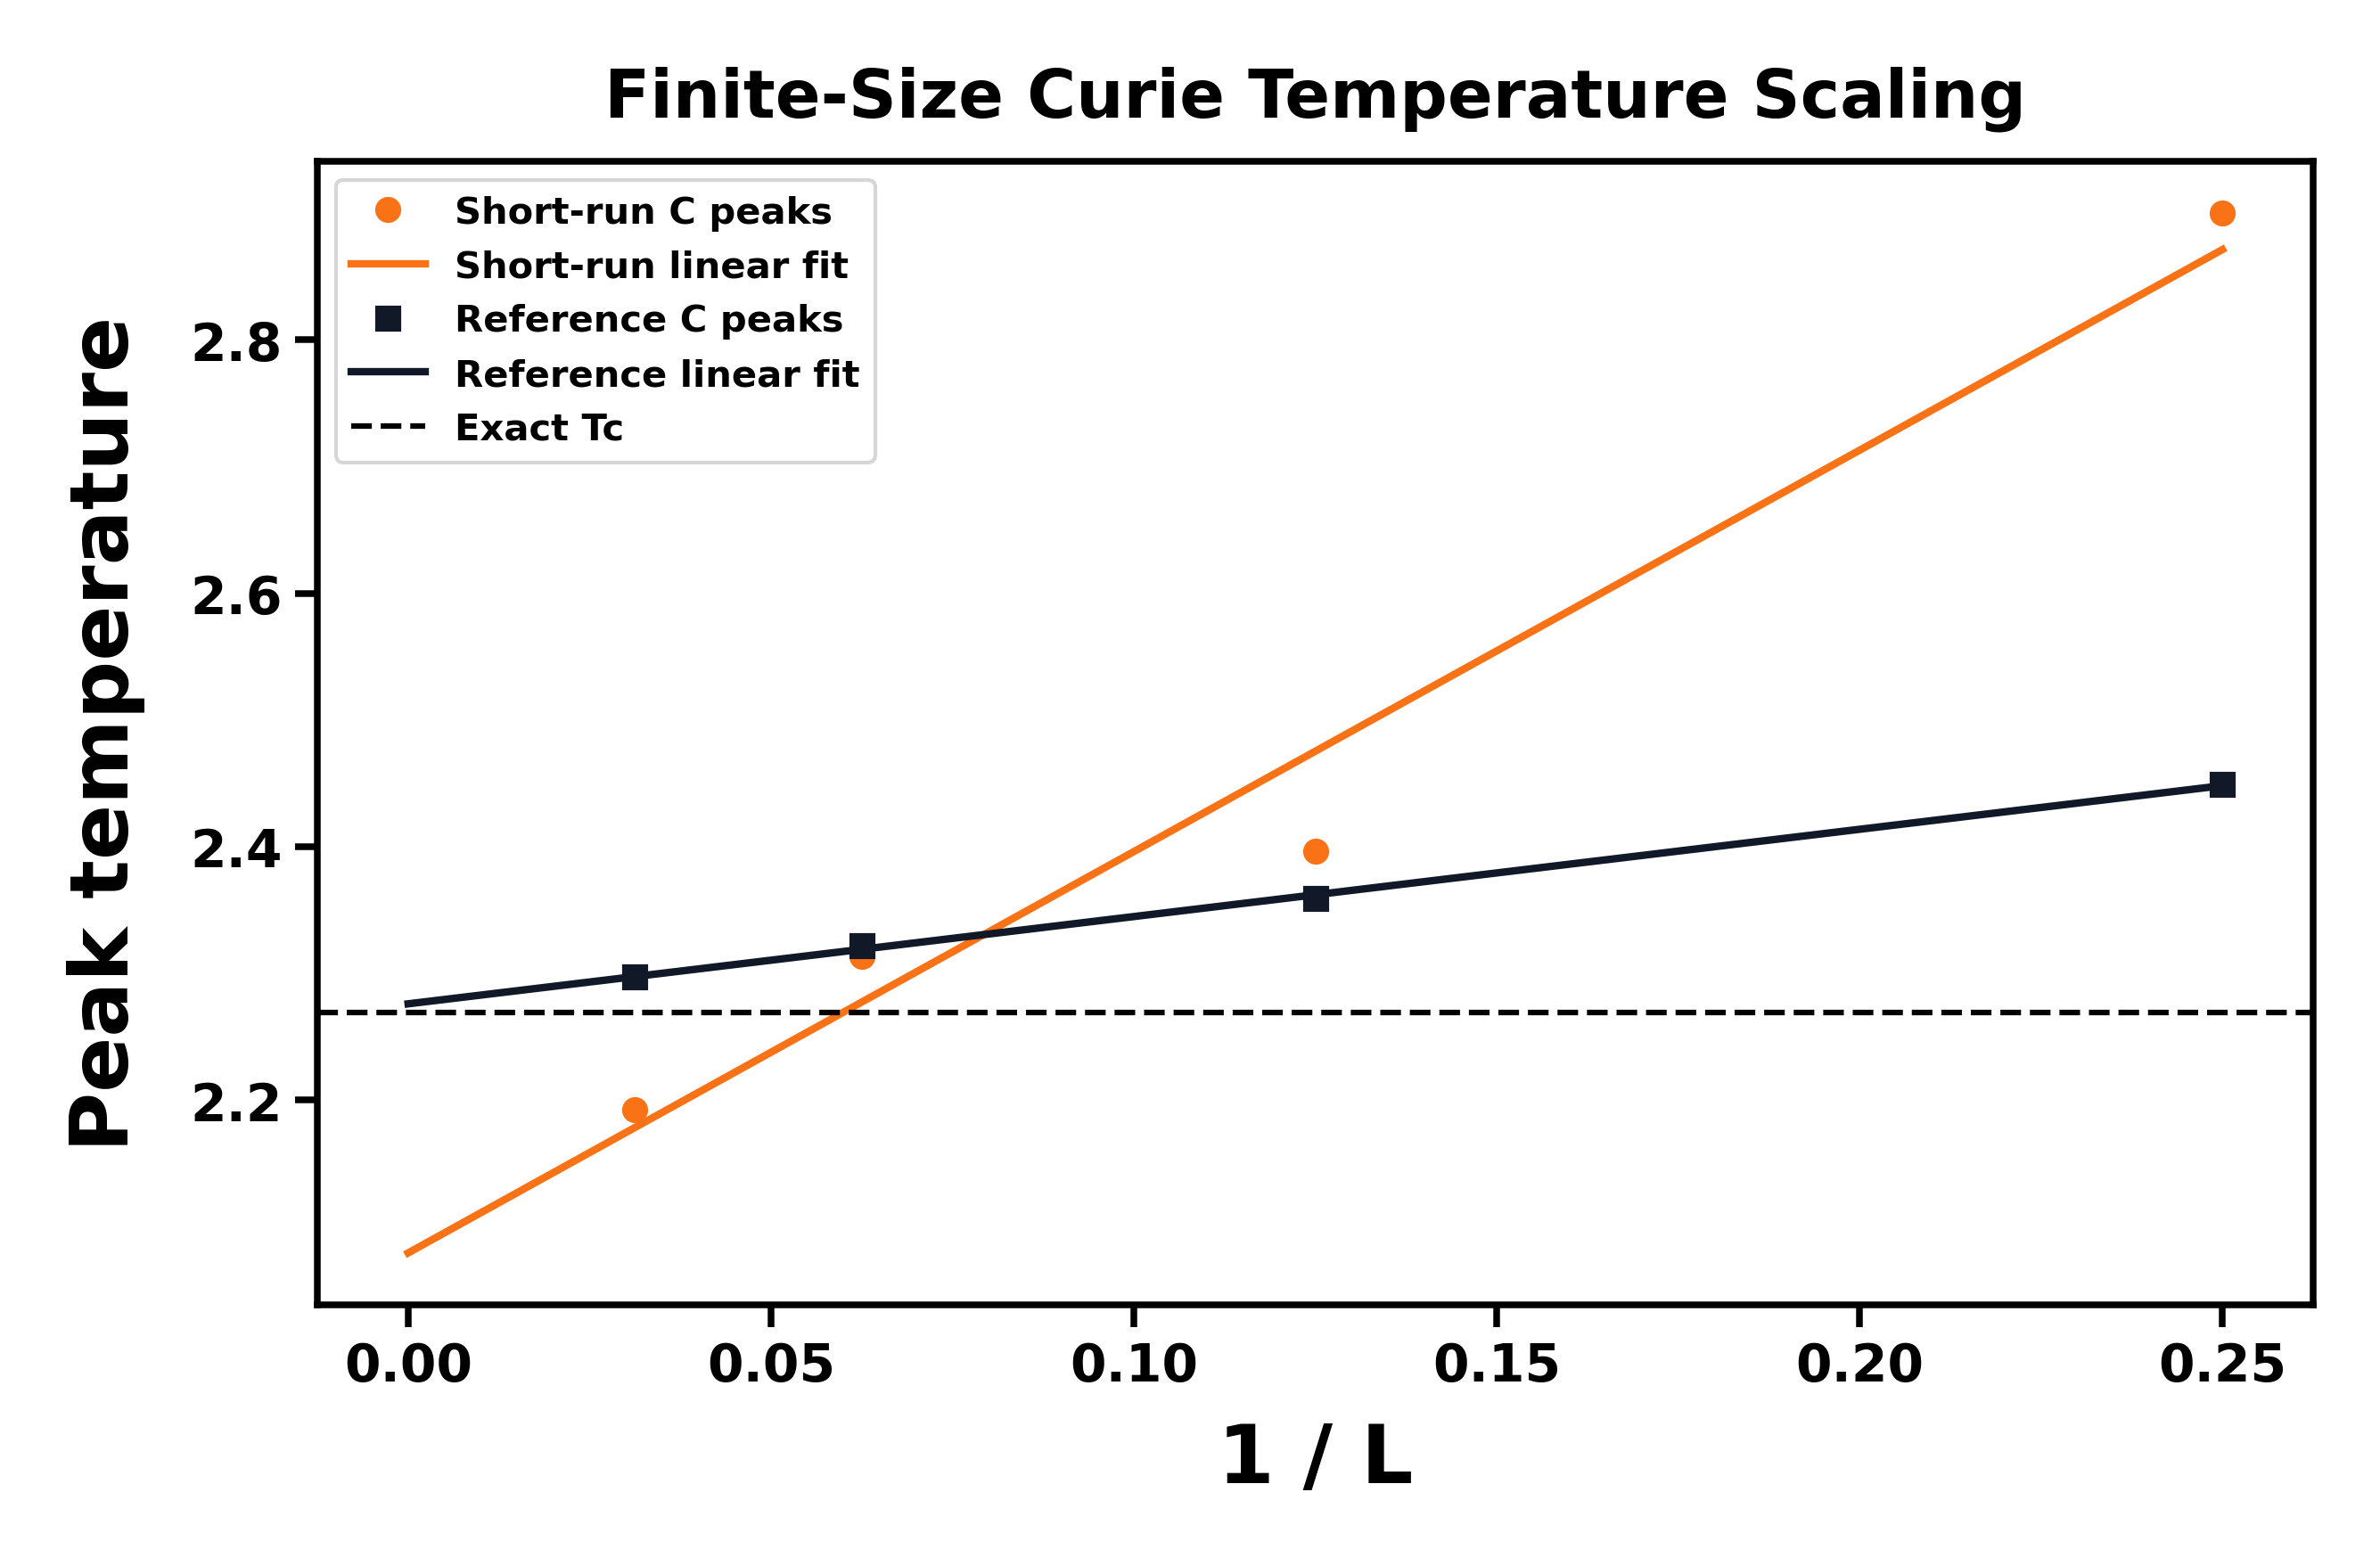
\includegraphics[width=0.74\textwidth]{figures/fig_section8_curie_scaling.png}
  \caption{Reference heat-capacity peak scaling extrapolates close to the exact Curie temperature. The short-run heat-capacity fit is visibly more sensitive to peak-estimation noise.}
  \label{fig:si_curie_scaling}
\end{figure}

\clearpage
\begin{figure}[p]
  \centering
  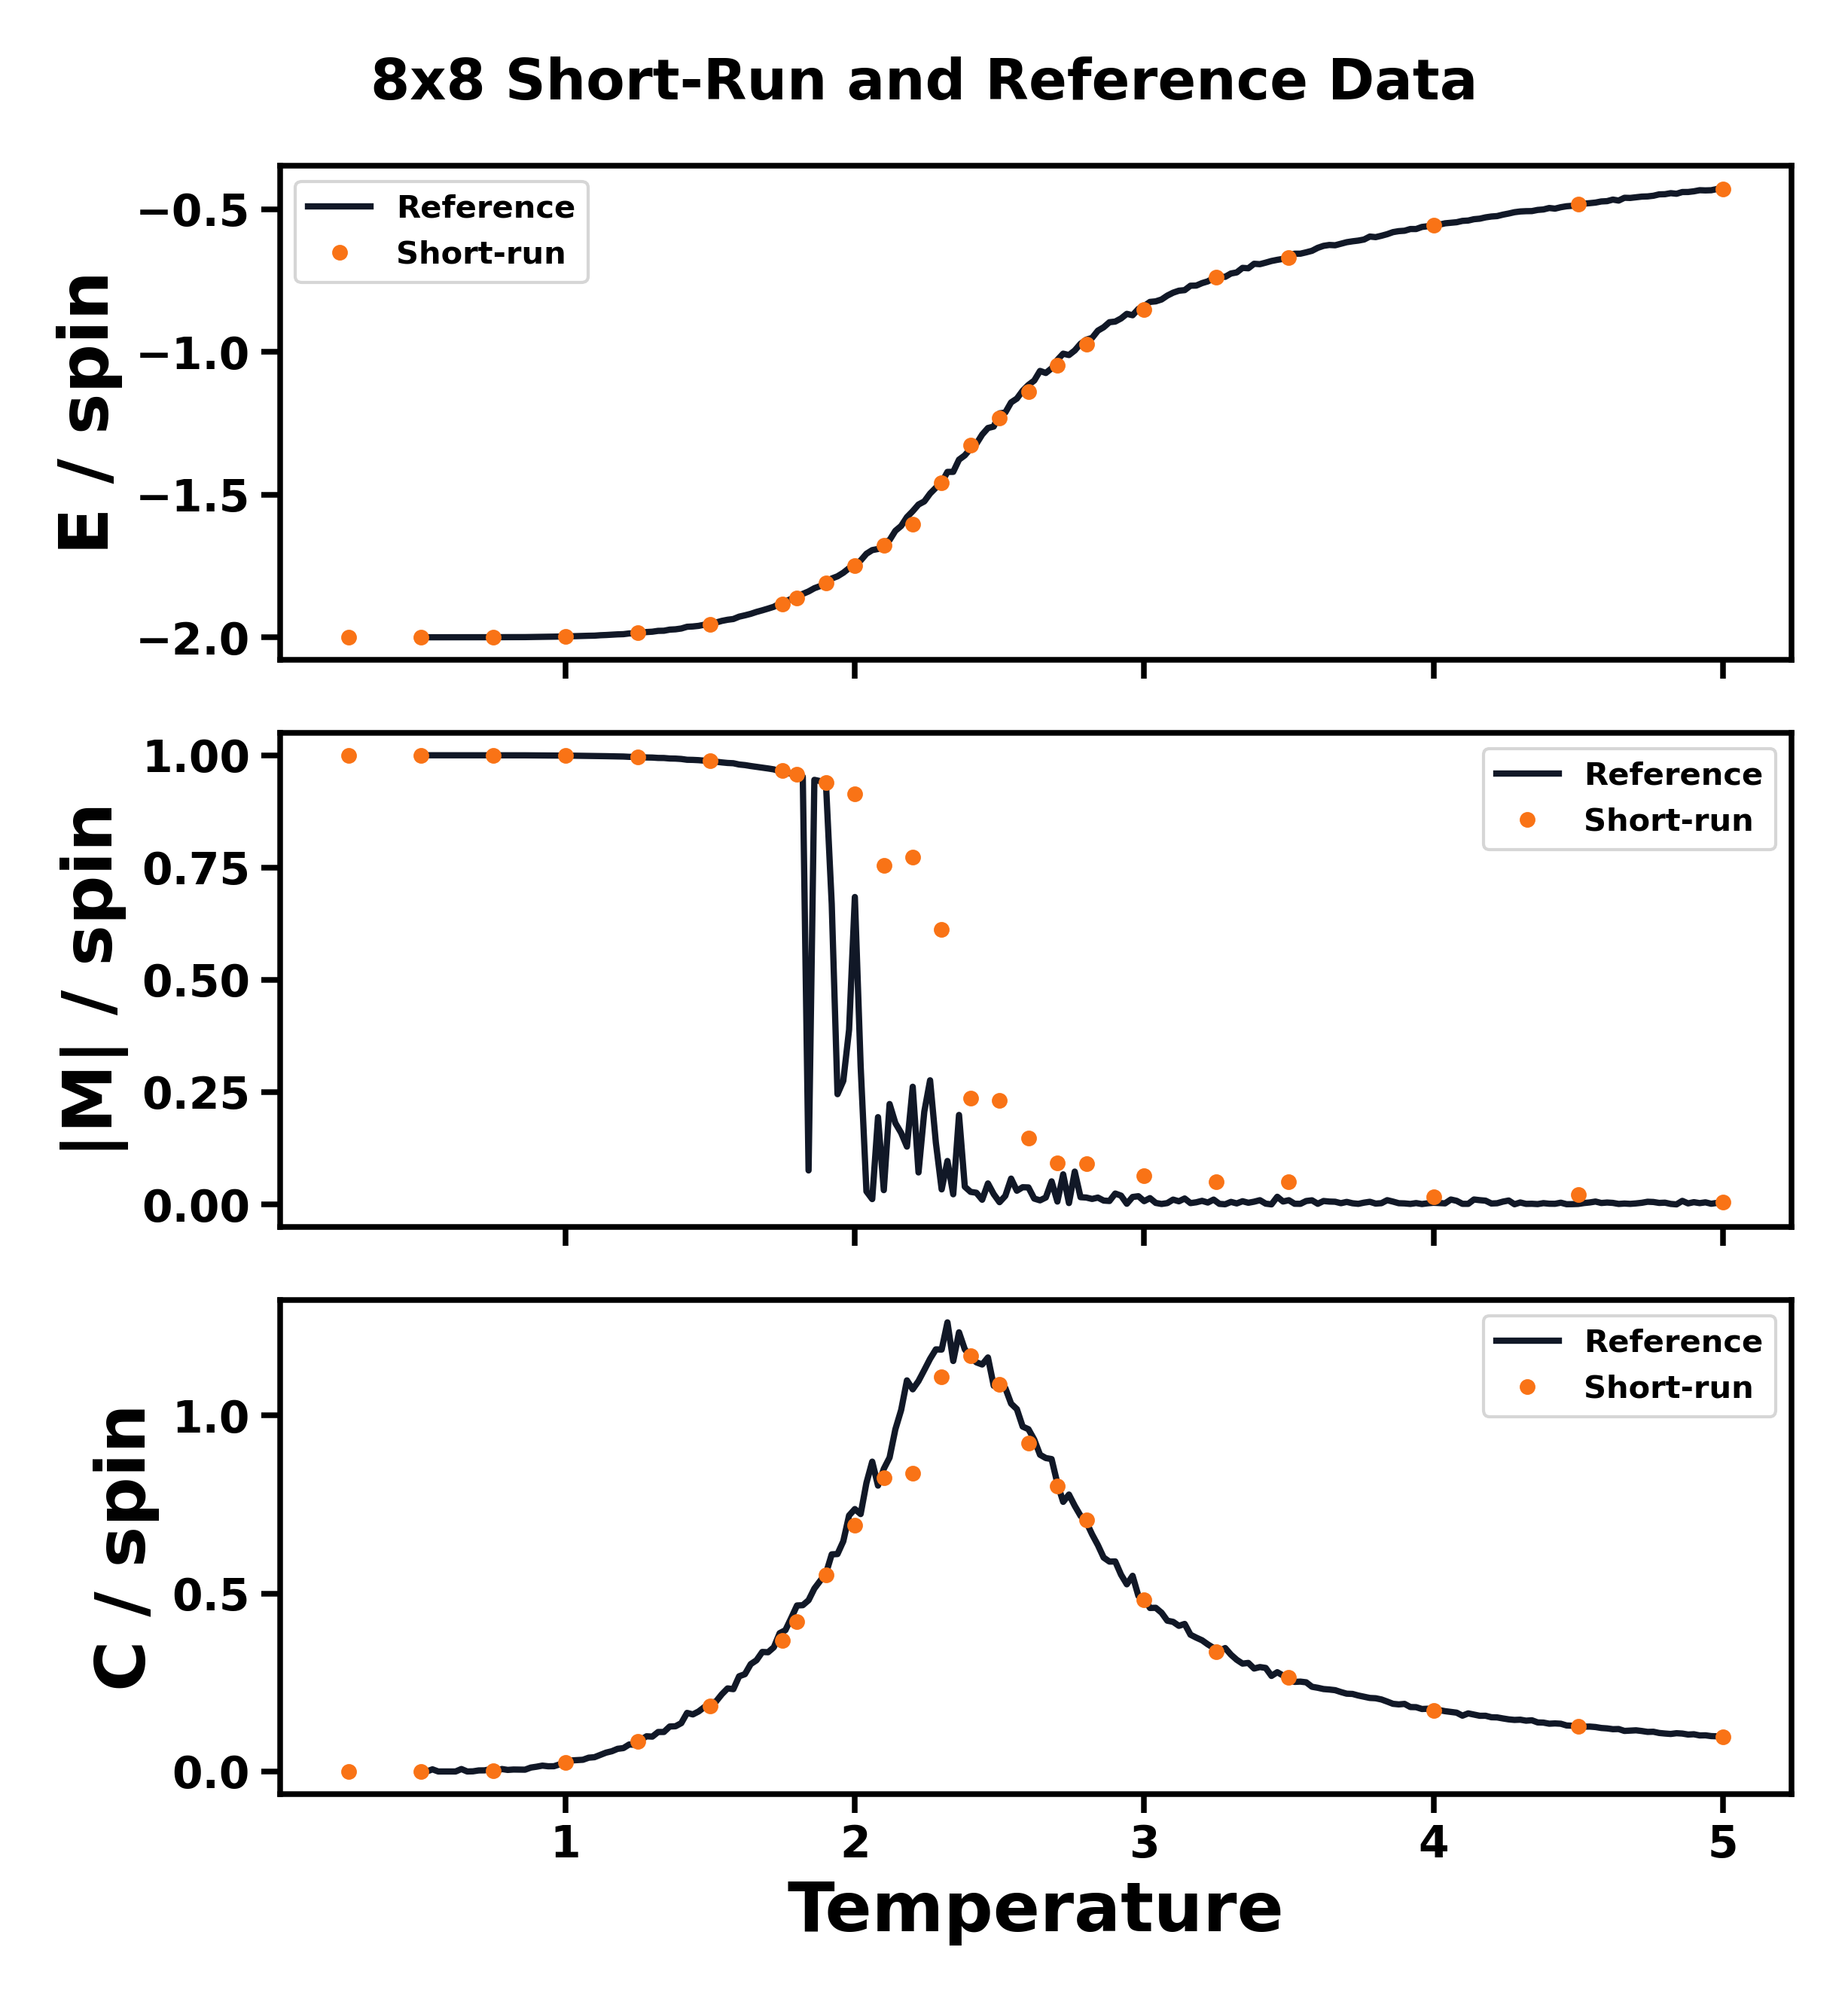
\includegraphics[width=0.86\textwidth]{figures/fig_section8_own_reference.png}
  \caption{Short-run and reference \(8 \times 8\) data agree in the main thermodynamic trends. The short-run simulation data are visibly noisier near the heat-capacity peak.}
  \label{fig:si_short_ref}
\end{figure}

\clearpage
\begin{figure}[p]
  \centering
  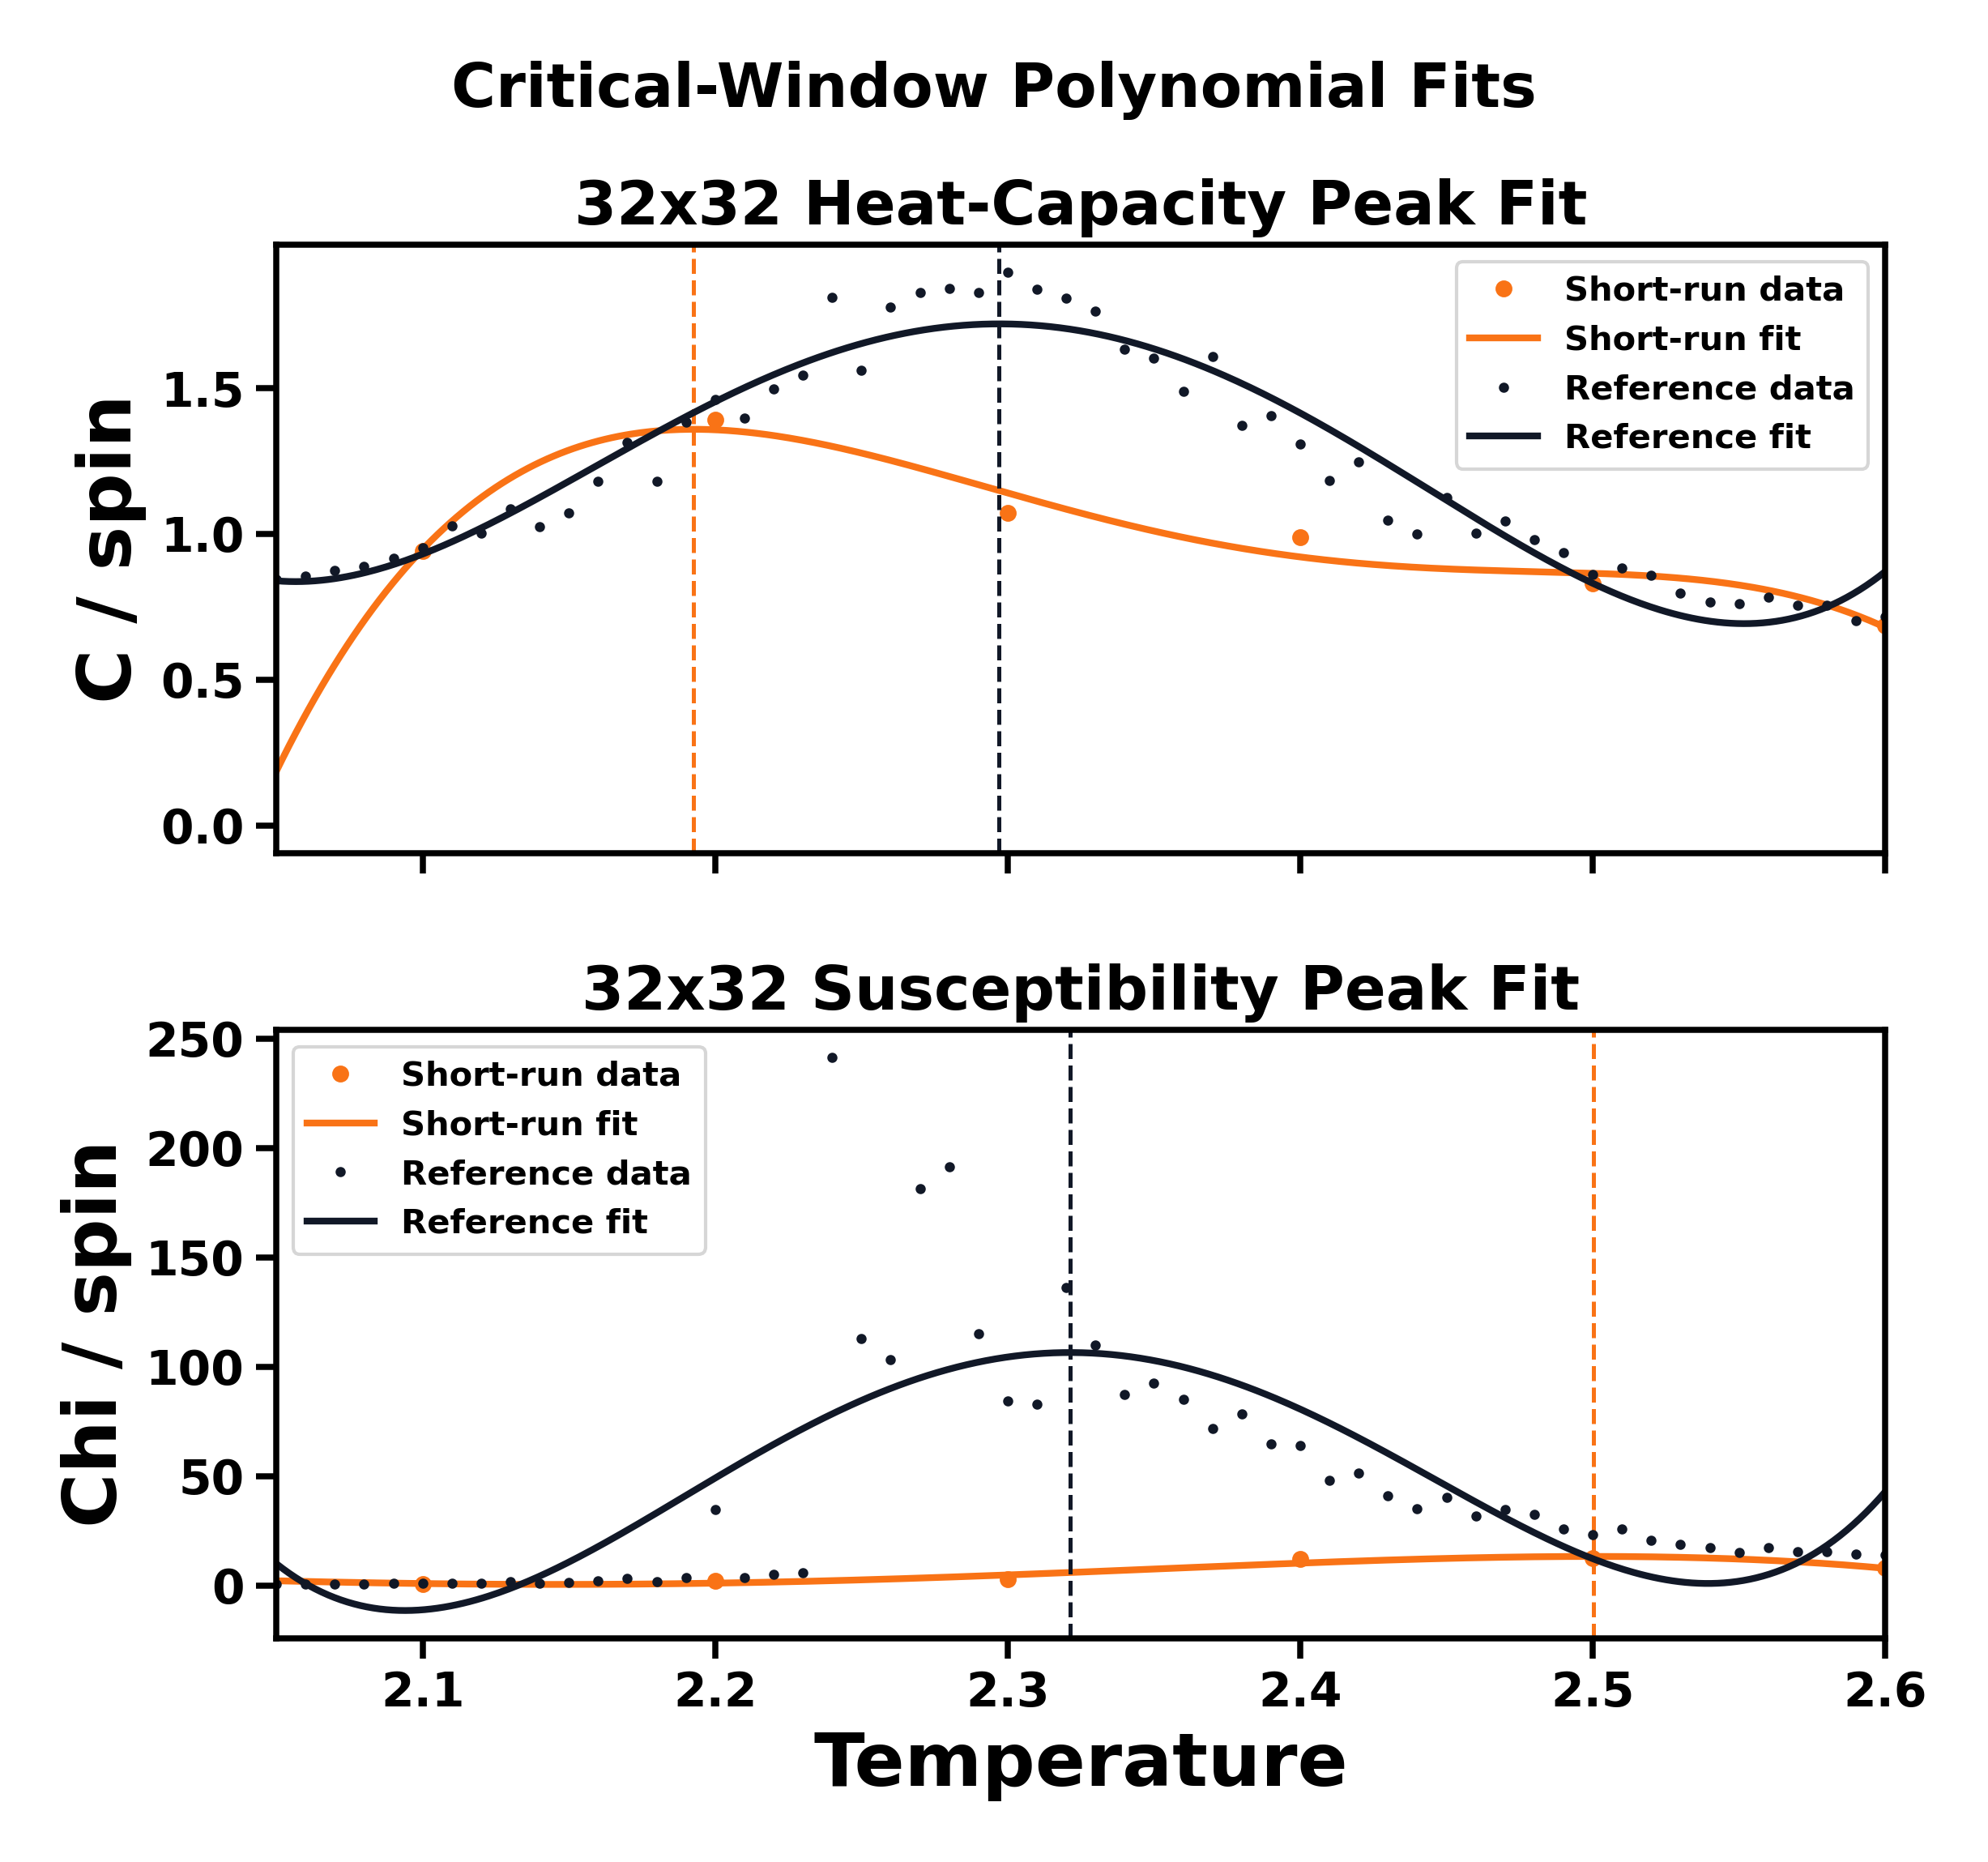
\includegraphics[width=0.84\textwidth]{figures/fig_section8_peak_fits.png}
  \caption{Polynomial peak fits are more stable for heat capacity than susceptibility at \(L=32\). Both observables were fitted in the selected critical window.}
  \label{fig:si_peakfit}
\end{figure}

\clearpage
\begin{figure}[p]
  \centering
  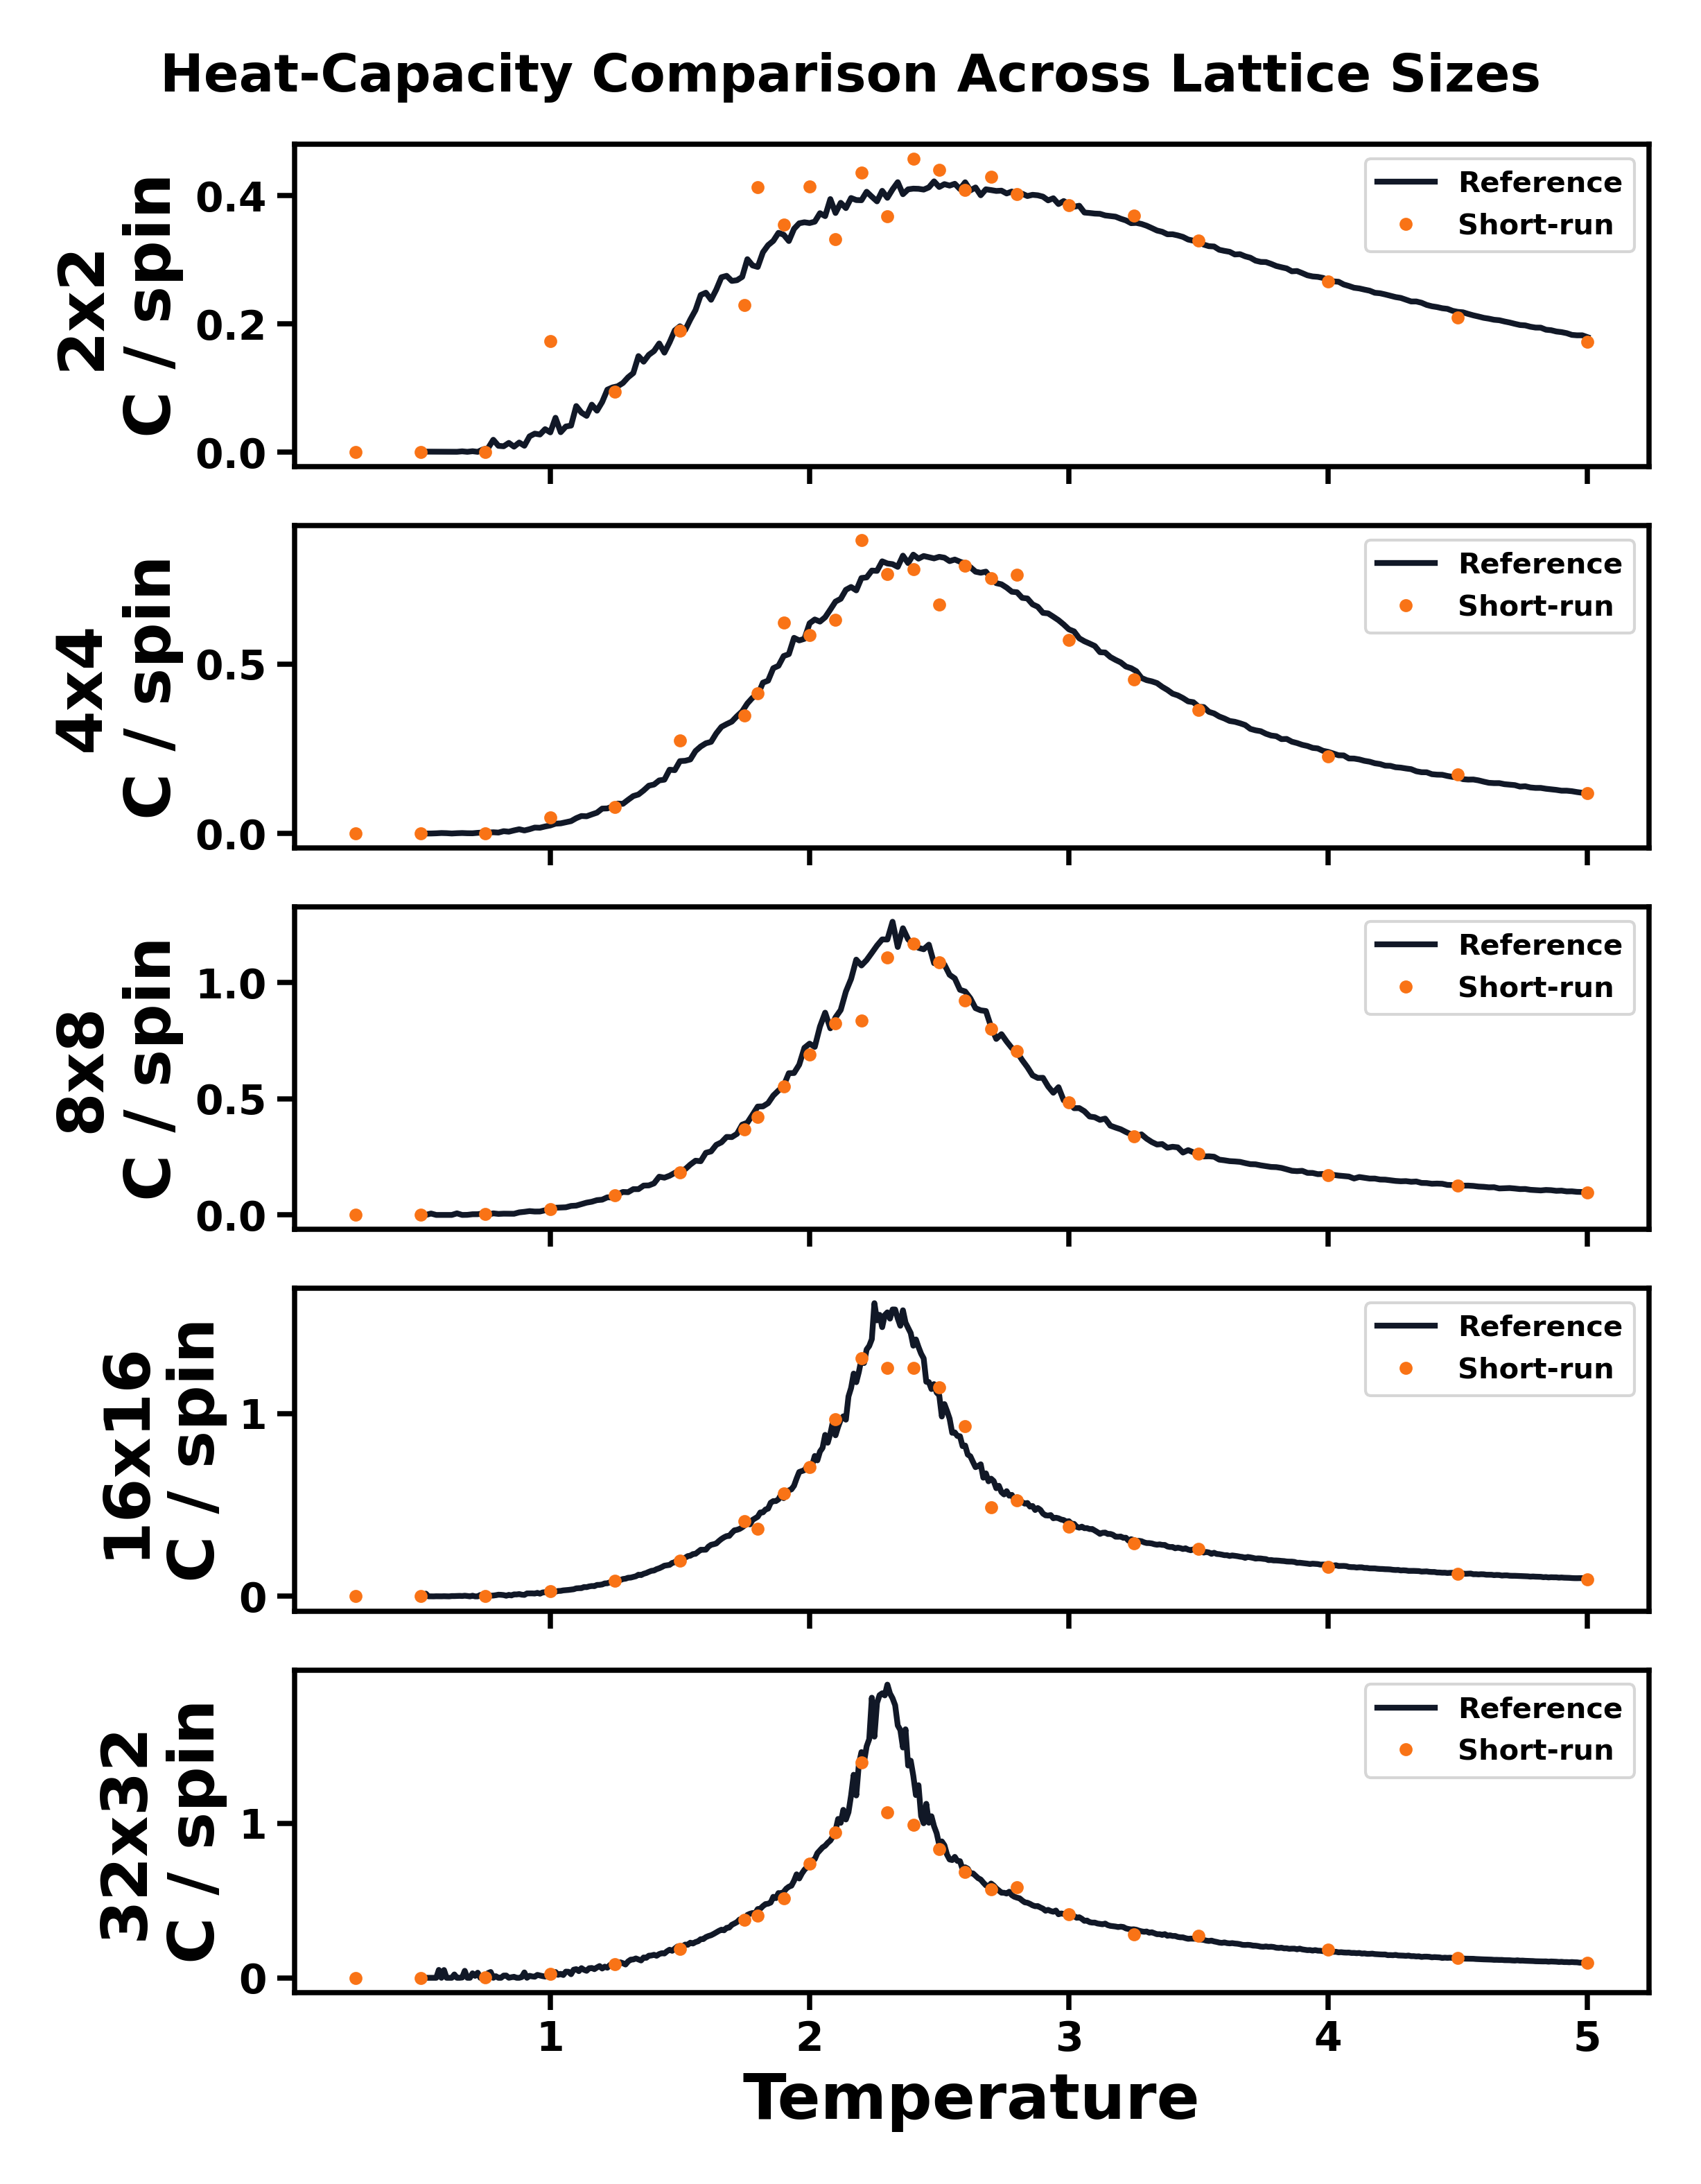
\includegraphics[width=0.86\textwidth]{figures/fig_section8_reference_heat_capacity.png}
  \caption{Reference heat-capacity data provide the smoothest peak sequence for Curie-temperature extrapolation. Longer simulations reduce peak noise relative to the short-run data.}
  \label{fig:si_reference_heat}
\end{figure}



\end{document}
